 \subsection{Doing Old Things with Micro-Genres}
 The link clustering procedure yields a ``new'' data set out of the old. Instead, of 2263 people choosing 20 vague macro-genre labels, we now have the same 2263 people, but their choices have been distilled and focused on 111 micro-genres. Since this is still a plain old survey data set, with people in the rows and micro-genres in the columns, we can perform some of the same old tricks (Factor Analysis, Latent Class Analysis, Multiple Correspondence Analysis) as before. But this time, the results will be more revealing, because we have honed in a bit closer upon the actual object that people made a taste judgment on and engage in their everyday musical listening practices. In addition, applying old techniques in this new data is likely to yield insights (e.g., combinations and classifications of micro-genres) that will not simply reproduce the standard findings of the past (e.g., clumping of vague macro-genre labels into even vaguer ``discourses'' like highbrow, pop, folk, and the like). 
 
 To show this, Figure~\ref{fig:mca-micro} displays what happens when we subject the new $2263 \times 111$ matrix to Multiple Correspondence Analysis. Because now we have 111 points (positive ``yes'' modalities) to worry about, I used hierarchical clustering on the MCA dimensions to clump the micro-genre points in the MCA space. Labels rendered in the same color are in the same cluster, suggesting that people tend to choose them together.  
 
 Note that the resulting picture (compared to Figure~\ref{fig:mca}) is now richer and more complex. Micro-genres trade focus for ``legibility'' at least when it comes to vague macro-genre clumps. However, this does not mean that there no interpretable results. On the contrary, it just means that there are \textit{more} interpretable results. For instance, take the clump of genres that dominates the first (horizontal) dimension of the MCA space micro-genre classification. Here, we see all the macro-genre labels represented in close proximity (indicating people tend to choose all these micro-genres in tandem. The micro-genres in this region of the space (as given by their low number designation) tend to have the largest audiences of their kind (with signal exceptions such as Rap, Country, and Jazz). This, therefore indicates micro-genres that go together due to a rather indiscriminate mixing of styles, indicative of a \textit{type} (but not the only type) of ``omnivorousness.'' 
 
  \begin{figure}[ht!]
 \centering
 \includegraphics[width=0.9\textwidth]{Figs/Link Clust/micro-genre-mca.png}
 \caption{Multiple Correspondence Analysis of Micro-Genre Data. Upper panel shows the Euclidean space formed by the first two dimensions, and the lower panel shows the space corresponding to the third and fourth dimensions. Micro-genres are hierarchically clustered (using Ward's criterion) into 17 clusters (see inset) based on their proximity in the four-dimensional MCA space. Micro-genre labels in the plot belonging to the same cluster are rendered in the same color.}
  \label{fig:mca-micro}
 \end{figure}
 
 Other regions display more focused clumpings of micro-genre styles, but ones that are not easily interpretable using the usual macro-categories. Toward the top of the upper panel, we see a combination of genres usual classified as ``contemporary'' or ``youth'' but also containing Classic Rock. Immediately below this clump, we see a three-micro genre cluster featuring both Classic and contemporary rock styles. In the lower panel of the figure, showing the space formed by the third and fourth dimensions, we see other interesting micro-genre mixtures. Toward the top, a micro-genre cluster composed of traditional ``high status'' genres like Classical music, but also featuring two country micro-genres and classic rock. As we will see below, this Classical micro-genre (``Classical\_3''), tends to feature individuals who do not mind making many choices. 
 
\section{Demographic Profiles of Micro-genre Communities}
We could continue trying to derive novel ``discourses'' of taste by looking at micro-genre clumps in the MCA space. Suffice to say that these are probably not going to look like the ones that have usually been noted in the literature (although some might). However, as noted, the core feature of the link clustering algorithm for discovering genre communities is that takes somewhat fuzzy and vaguely defined macro-genre labels (e.g., ``Classical,'' ``Classic Rocks/Oldies,'' ``Country,'' or ``Pop'') and decomposes them into more focused micro-genre communities. The remaining question is whether these micro-genres are valid, in terms of attracting systematically different types of people. To show this, I follow the venerable principle of audience segmentation to verify the validity of the procedure to discover interpretable micro-genres \citep{peterson92}. 

\subsection{Classical}

 \begin{figure}[ht!]
 \centering
 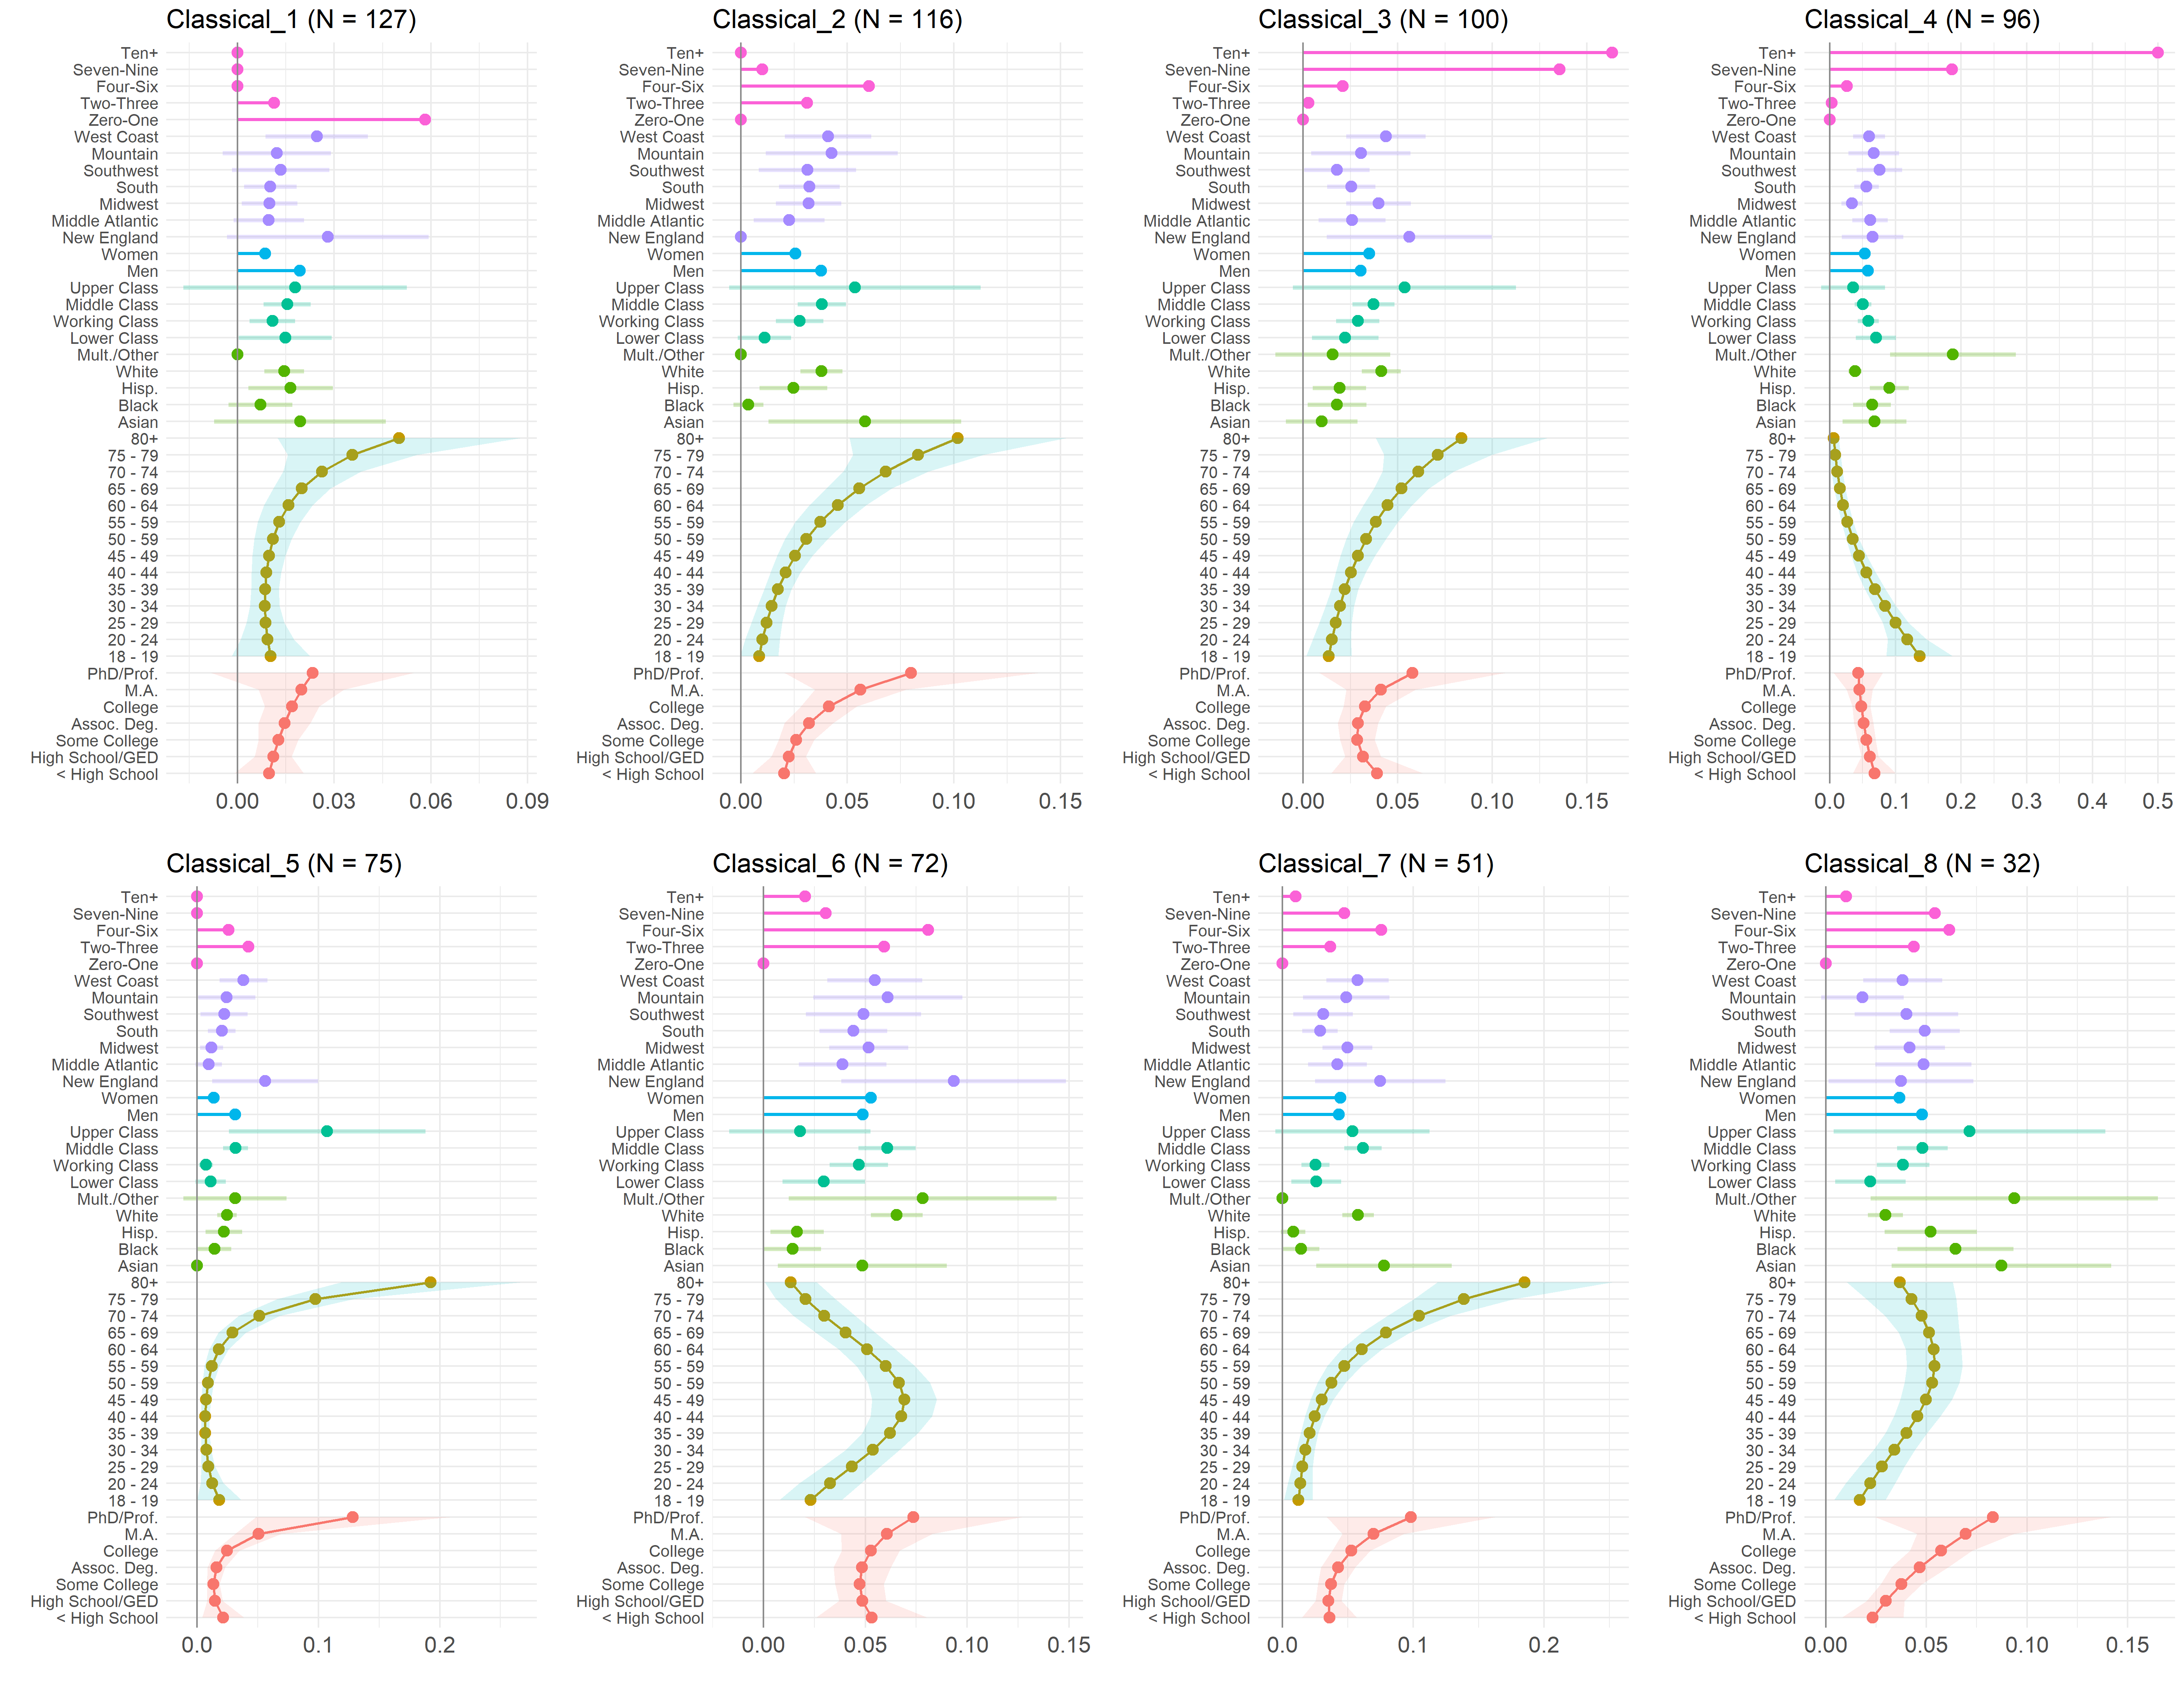
\includegraphics[width=1.0\textwidth]{figs/demog-plots/Classical.png}
 \caption{}
  \label{fig:classical}
 \end{figure}
 
Figure~\ref{fig:classical} shows the demographic profiles for the eight ``Classical'' micro-genres discovered by the link clustering procedure. Demographic profiles are depicted as the predicted probabilities (and associated confidence intervals around these estimates) obtained from a logistic regression of the relevant sociodemographic characteristic (in this case, education (red), age (mustard), ethnoracial identification (green), subjective class identification (teal), gender (blue), and region of residence (purple), along with a categorical breakdown of the total number of genres chosen (pink)) against the log odds of having chosen that particular micro-genre \citep{king_etal00}. 

 \begin{figure}[ht!]
 \centering
 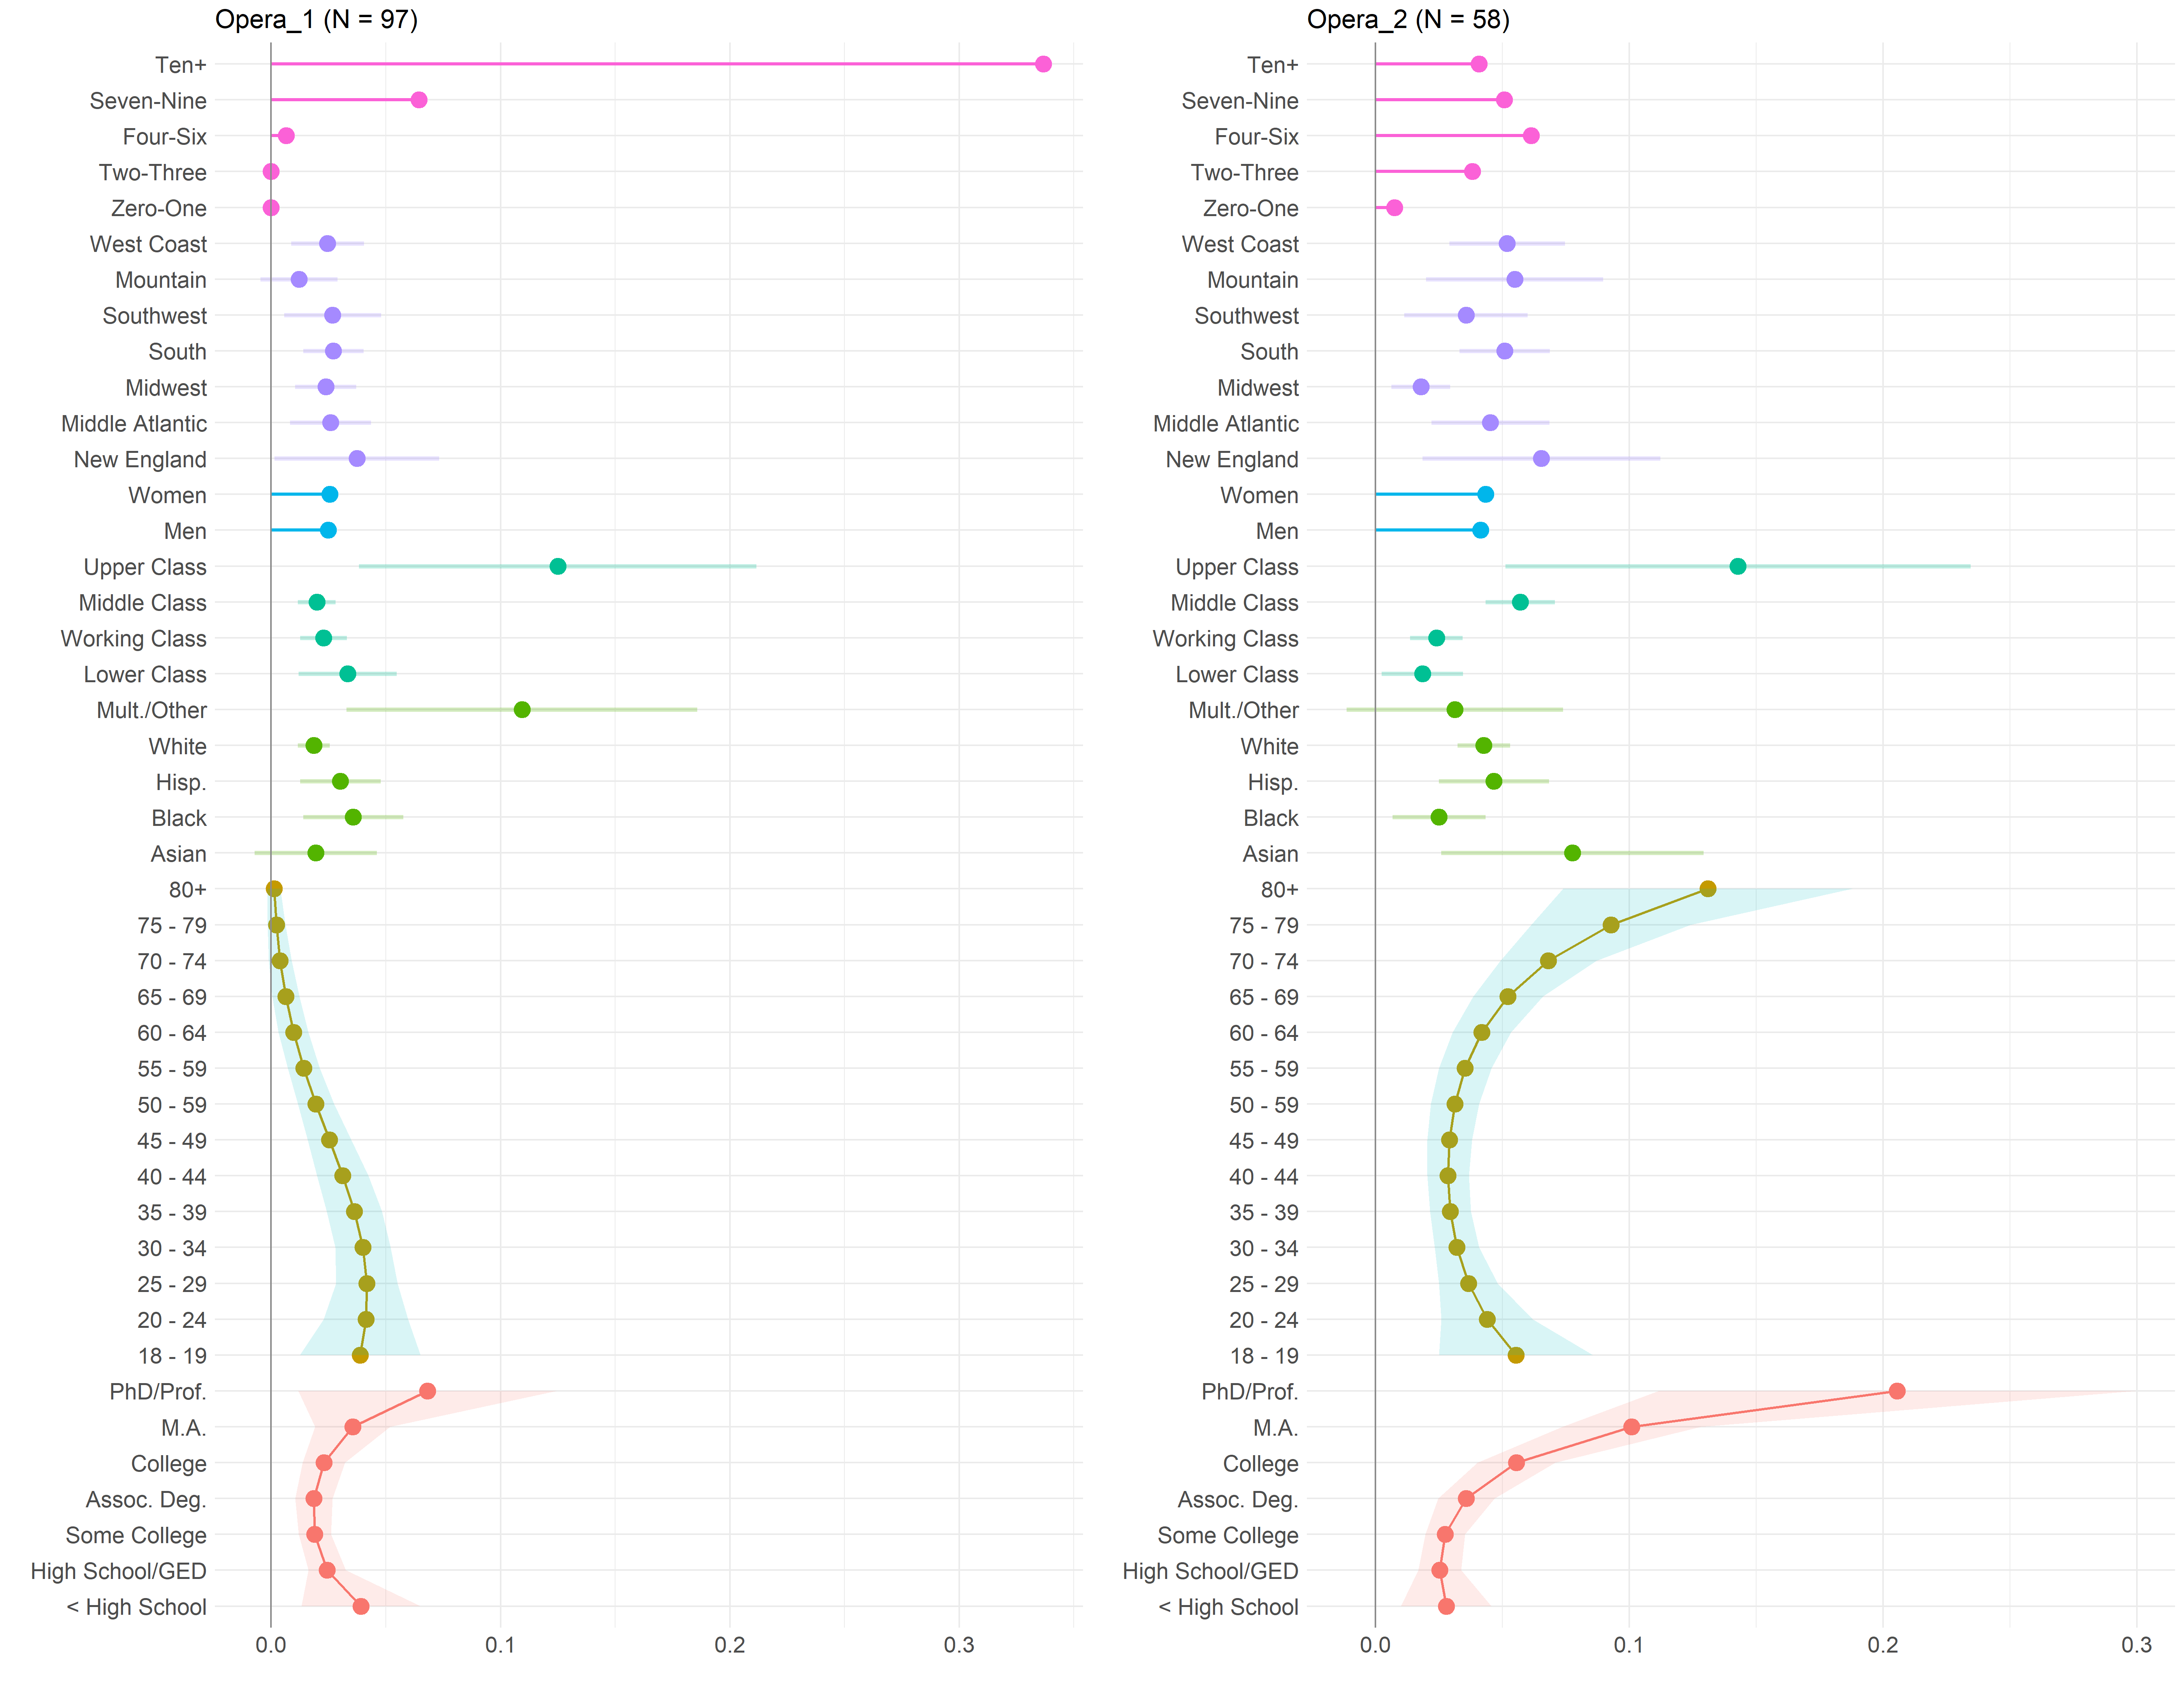
\includegraphics[width=1.0\textwidth]{figs/demog-plots/Opera.png}
 \caption{}
  \label{fig:opera}
 \end{figure}

The first Classical micro-genre ($N=127$), picks up a micro-genre that appeals to the Classical music ``univore.'' This person is likely to be old, likely to be a man living in a New England state; some of us have perhaps met this person and can imagine what version of Classical music this is (likely to be the most stereotyped around the established canon \citep{kremp10}). The second Classical micro-genre ($N = 116$,) seems like what is seen as the prototypical consumer of Classical music \citep{lizardo_skiles16}. This person is likely to be older, hold and advanced degree, be white and identify as middle class. Interestingly, other micro-genre variations of Classical picked by the analysis (3, 5, 7, and 8) capture variations of Classical music that also appeal to older, highly educated people; interestingly, these other Classical musics differ from the last variant with respect to the other markers of social position. The third Classical micro-genre (($N = 100$) is characterized by extreme omnivorousness by volume; the fifth micro-genre ($N = 75$) is distinguished by the fact that the people who choose it are men who are also likely to identify as ``Upper Class'' (a rare designation in the U.S. case). The seventh micro-genre ($N = 51$) is inordinately likely to be consumed by Asian respondents, while the eighth, and smallest, micro-genre ($N = 32$) is more likely to attract nonwhite respondents. The link clustering approach can thus recover micro-genre communities that appeal to ethnoracial minorities even in the case of a stereotypically ``white'' macro-genre label such as Classical \citep{lizardo_skiles16}. The remaining Classical micro-genres have demographic profiles that deviate from the stereotypical Classical music consumer. People attracted to the fourth Classical micro-genre ($N = 96$) are young omnivores, while those choosing the sixth variation ($N = 72$) are middle-aged New Englanders who are either white or multiracial. 

\subsection{Opera}

Not all macro-genre labels are decomposed into a multiplicity of micro-genres. Take the case of Opera, shown in Figure~\ref{fig:opera}. The link clustering procedure discovers only two micro-genre variations in this case. A version chosen by omnivorous respondents who choose a multiplicity of other genres (and who are also younger, identify as upper class and are likely to be multiracial)and a micro-genre that looks a look like the stereotype; older, highly educated, upper/middle-class person. This suggests that, save for the version chosen by omnivores, the macro-genre label ``Opera'' already gets at a relationally focused micro-genre. A situation very different from ``Classical.'' This puts into question the common strategy of treating these two macro-genre labels as equivalent indicators of an overall ``highbrow'' dispositions. As we have seen, while some versions of Classical do fit that bill in terms of their sociodemographic profile, others certainly do not. 

 \begin{figure}[ht!]
 \centering
 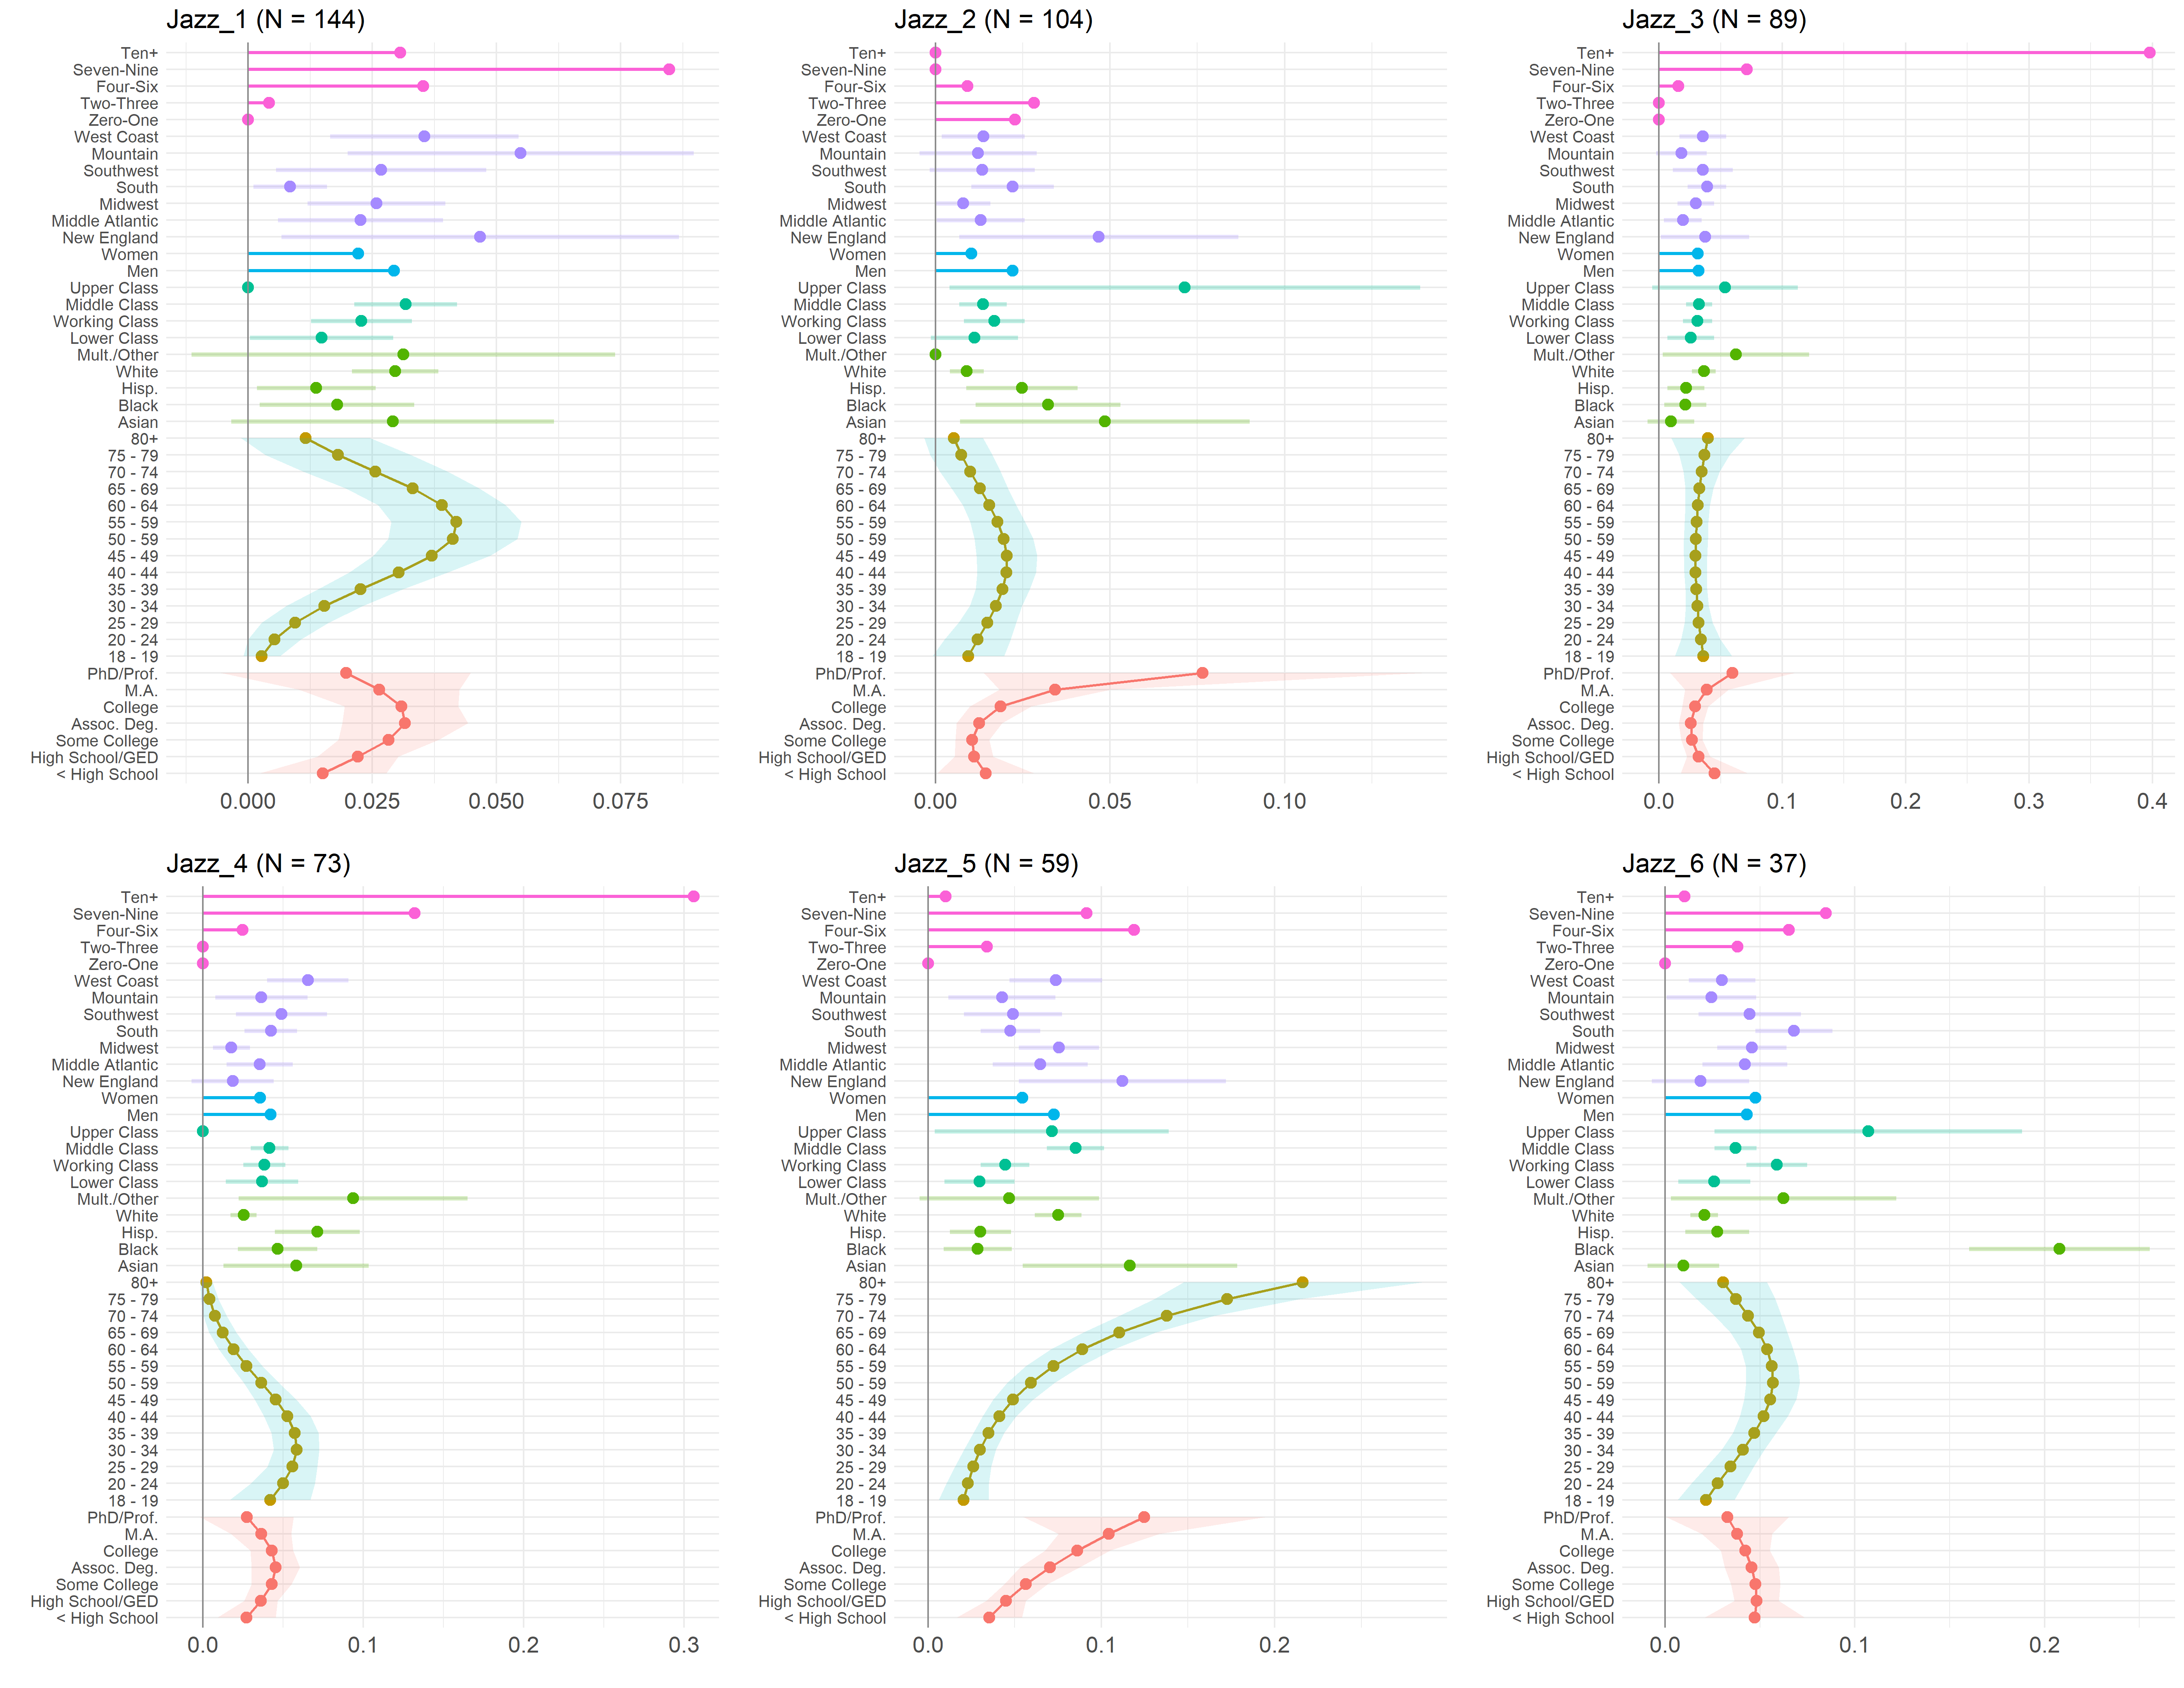
\includegraphics[width=1.0\textwidth]{figs/demog-plots/Jazz.png}
 \caption{}
  \label{fig:jazz}
 \end{figure}
 
 \subsection{Jazz}

The case of Jazz is an instructive one for the link clustering procedure, given the complex historical trajectory of the genre. It began as an ``artistic'' (expert performer-driven and focused) genre in the Black art world in the early 20th century, diffusing into both Black middle and working-class consumer communities and white aesthetic (both performer and consumer-driven) circles by mid-century, and then legitimized as a high art form in conservatories later on \citep[see][]{lopes02}. Accordingly, ``Jazz'' has always been suspected of being the ultimate multivocal macro-genre labels, condensing complex dynamics of ethnoracial, social class, and generational status. Whatever it may be, ``Jazz'' is simply not a single kind of thing and thus represents one of the linchpins of the macro-genre label critique. 

The link clustering analysis shown in Figure~\ref{fig:jazz}, agrees; but with a caveat. Split into relationally structured micro-genres, Jazz is not a single thing, but neither is it an unruly multiplicity of unrelated things. Instead, it seems to be a small collection, summarizing in the synchrony of respondent choices in 2012, the complex history alluded to. In that respect, the micro-genre approach can tell the difference between the Jazz variant appealing to mainly white, older, highly educated New Englanders (version 5, $N = 59$), perhaps the aestheticized and institutionalized conservatory version, and the one whose primary marker is appeal to middle-aged Black respondents who mainly reside in the American south, but otherwise lacking a strong education gradient (version 6, $N = 37$). Interestingly, there is also a version of Jazz (version 3, $N = 104$) that has a strong education gradient and a relatively weak relationship with age, that primarily appeals to non-white audiences. This version is also the most gendered, and univorous being more likely to be engaged in by men who do not choose a wide variety of other genres. Finally, in addition to two omnivorous versions (versions 3, 4) we discover one ultimate ``middlebrow'' version of Jazz, largest of micro-genre communities identified (version 1,$N = 144$); this genre appeals to middle-aged respondents with equally middling education levels who identify as middle class; Jazz as ``cultural goodwill'' \citep{bourdieu84}.

 \begin{figure}[ht!]
 \centering
 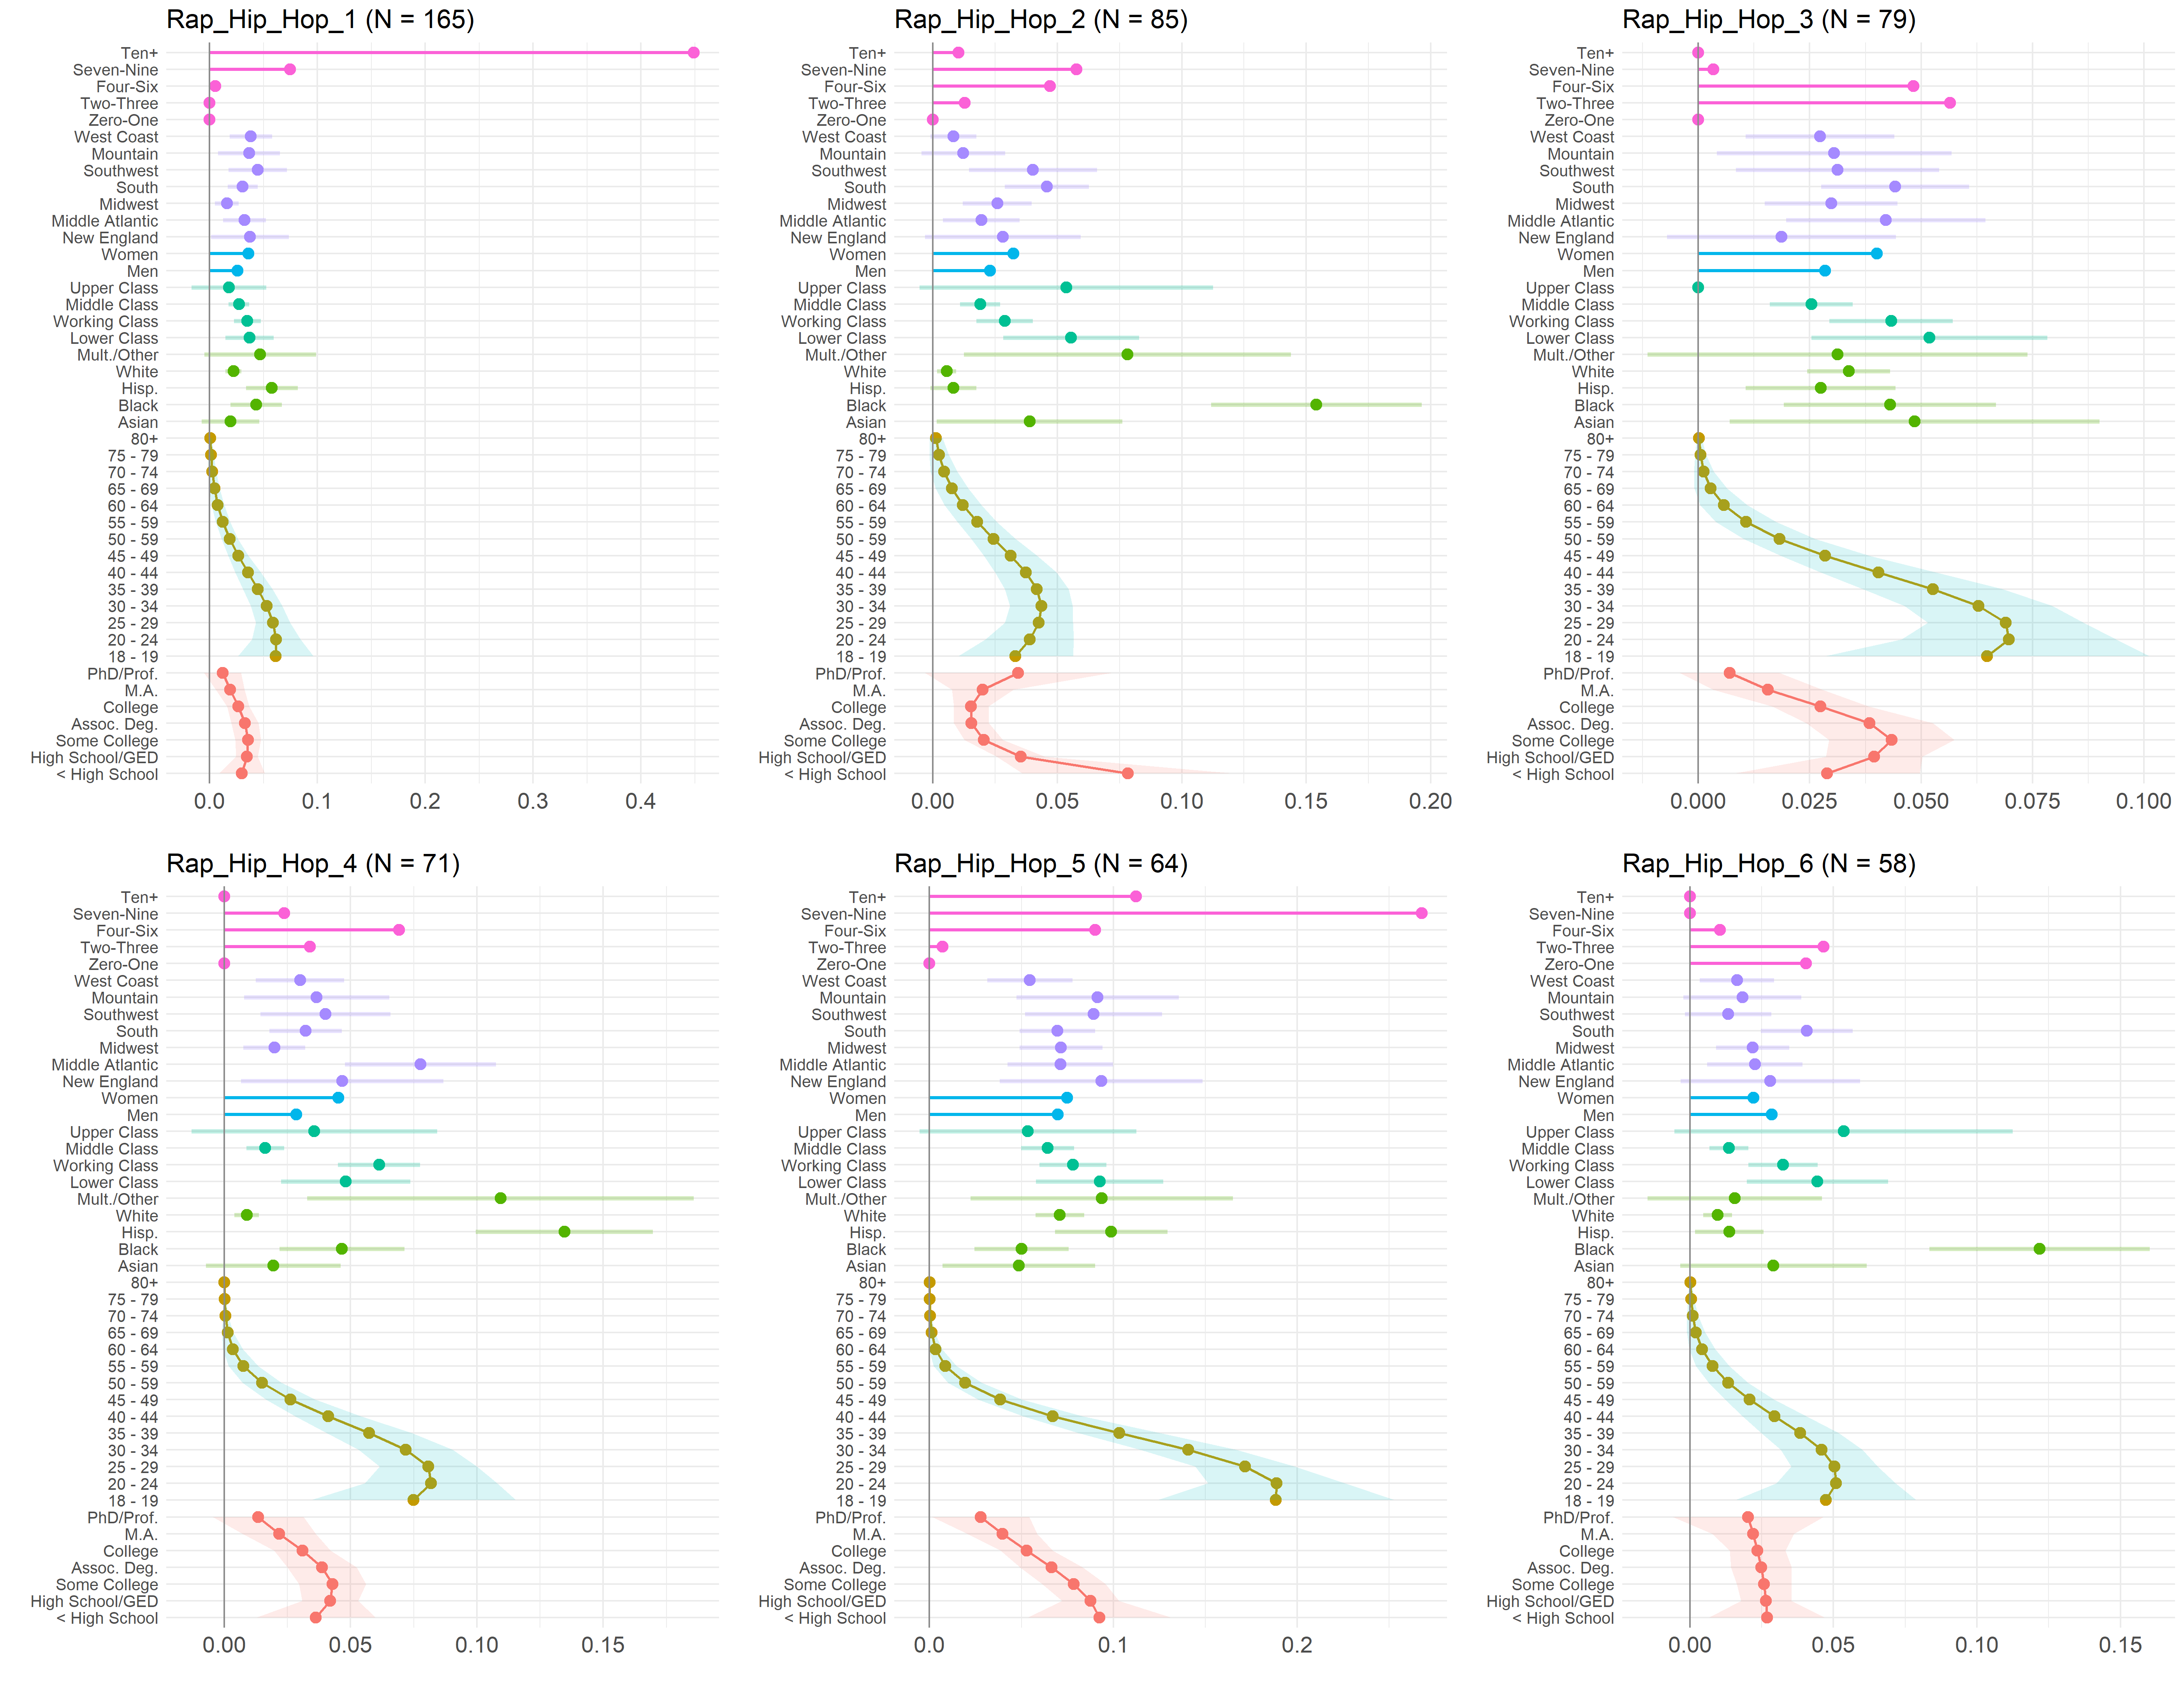
\includegraphics[width=1.0\textwidth]{figs/demog-plots/Rap_Hip_Hop.png}
 \caption{}
  \label{fig:rap}
 \end{figure}
 
\subsection{Rap/Hip Hop}
While not having as long a career as Jazz or the Blues, Rap/Hip Hop has also endured vicissitudes as its sociological genre bases have been transformed from its inception as a ``scene'' genre in the late 1970s, followed by a slow proliferation into geographically segmented scenes in the 1980s and 1990s, its slow and hesitant uptake by industry during the same period, and its emergence as a full-fledged industry-backed ``pop'' genre in the 21st century. Throughout, however, the strong association of Rap with young, Black, male performers and associated audiences (a situation that is in the process of being undone in the last decade or so with the emergence of powerful, iconic women rap performers with a strong foothold in industry) is one that is hard to shake \citep{lizardo_skiles16}.

The micro-genre analysis, shown in Figure~\ref{fig:rap} discovers six variations, producing results that both support and contravene those expectations. Regarding the latter, none of the micro-variations of rap are strongly gendered, suggesting that this is not a powerful principle of audience segmentation here. On other hand, age/generation is such a powerful principle with rap audiences across all six micro-genres all of which are more likely to appeal to young people. The only difference is the {\em strength} of the age effect, being strongest for variations 1, 2, and 3 ($N=164$, $N=84$, and $N=78$, respectively), and weaker for 4, 5, and 6 ($N=70$, $N=63$, and $N=57$, respectively). Variation 1, featuring the largest audience size, also features the least ethnoracial differentiation (save for the ``most omnivorous'' variation 4), and a penchant to combine with other genres; this suggests that this variation picks up the ``industry'' version of Hip Hop that presents itself today as radio-friendly pop music. This seems to stand opposed to variation 6; this is the smallest rap micro-genre, it has the strongest tilt toward Black, young audiences, and features the lowest propensity to be combined with other genres. Variation 5 is just like this last one, except that it features a strong tilt toward audiences without a college degree and a higher propensity to mix with other genres. 

One issue, in the wake of the emergence of Rap and Hip Hop as general pop culture genres, is the extent to which some micro-variations appeal to non-Black audiences. The link clustering procedure can tell the difference, producing a micro-genre variation (2) that is much less likely to appeal to Black audiences and more likely to appeal to those who identify as ``Hispanic'' or ``multiracial'' (perhaps picking up ethnolinguistic variants of Hip Hop). In the same way, Neither variation 3 or 4 (along with 1 as already discussed) exhibit as strong a tilt toward Black audiences as 2, 5, and 6. Suggesting that audience segmentation along ethnoracial identity is strong within Rap/Hip Hop micro-genres despite the relatively weaker levels of segmentation along education or generational lines. 

\subsection{Gospel/Religious}
The macro-genre fuzzy label ``Gospel/Religious'' is a lot like Jazz, in the sense that analysts know that it mixes micro-genre variations with distinct racialized audiences. As shown in Figure~\ref{fig:gospel}, the link clustering approach breaks this confounding, discovering three variations of Gospel primarily engaged in by Black people (1, 3 and 5) and one that primarily appeal to white people (4, $N = 86$), all of whom are likely to live the American South. Two of the Black gospel communities are mainly differentiated by age, with version 3 to working-class adults, and version 4 mainly appealing to middle class older people; both Black and white Gospel/Religious micro-genres are more likely to be engaged in by women. Version 1 is a Black Gospel univore community, and version 5 $N = 103$ is the omnivore micro-genre variation (which exists for all genres).      

 \begin{figure}[ht!]
 \centering
 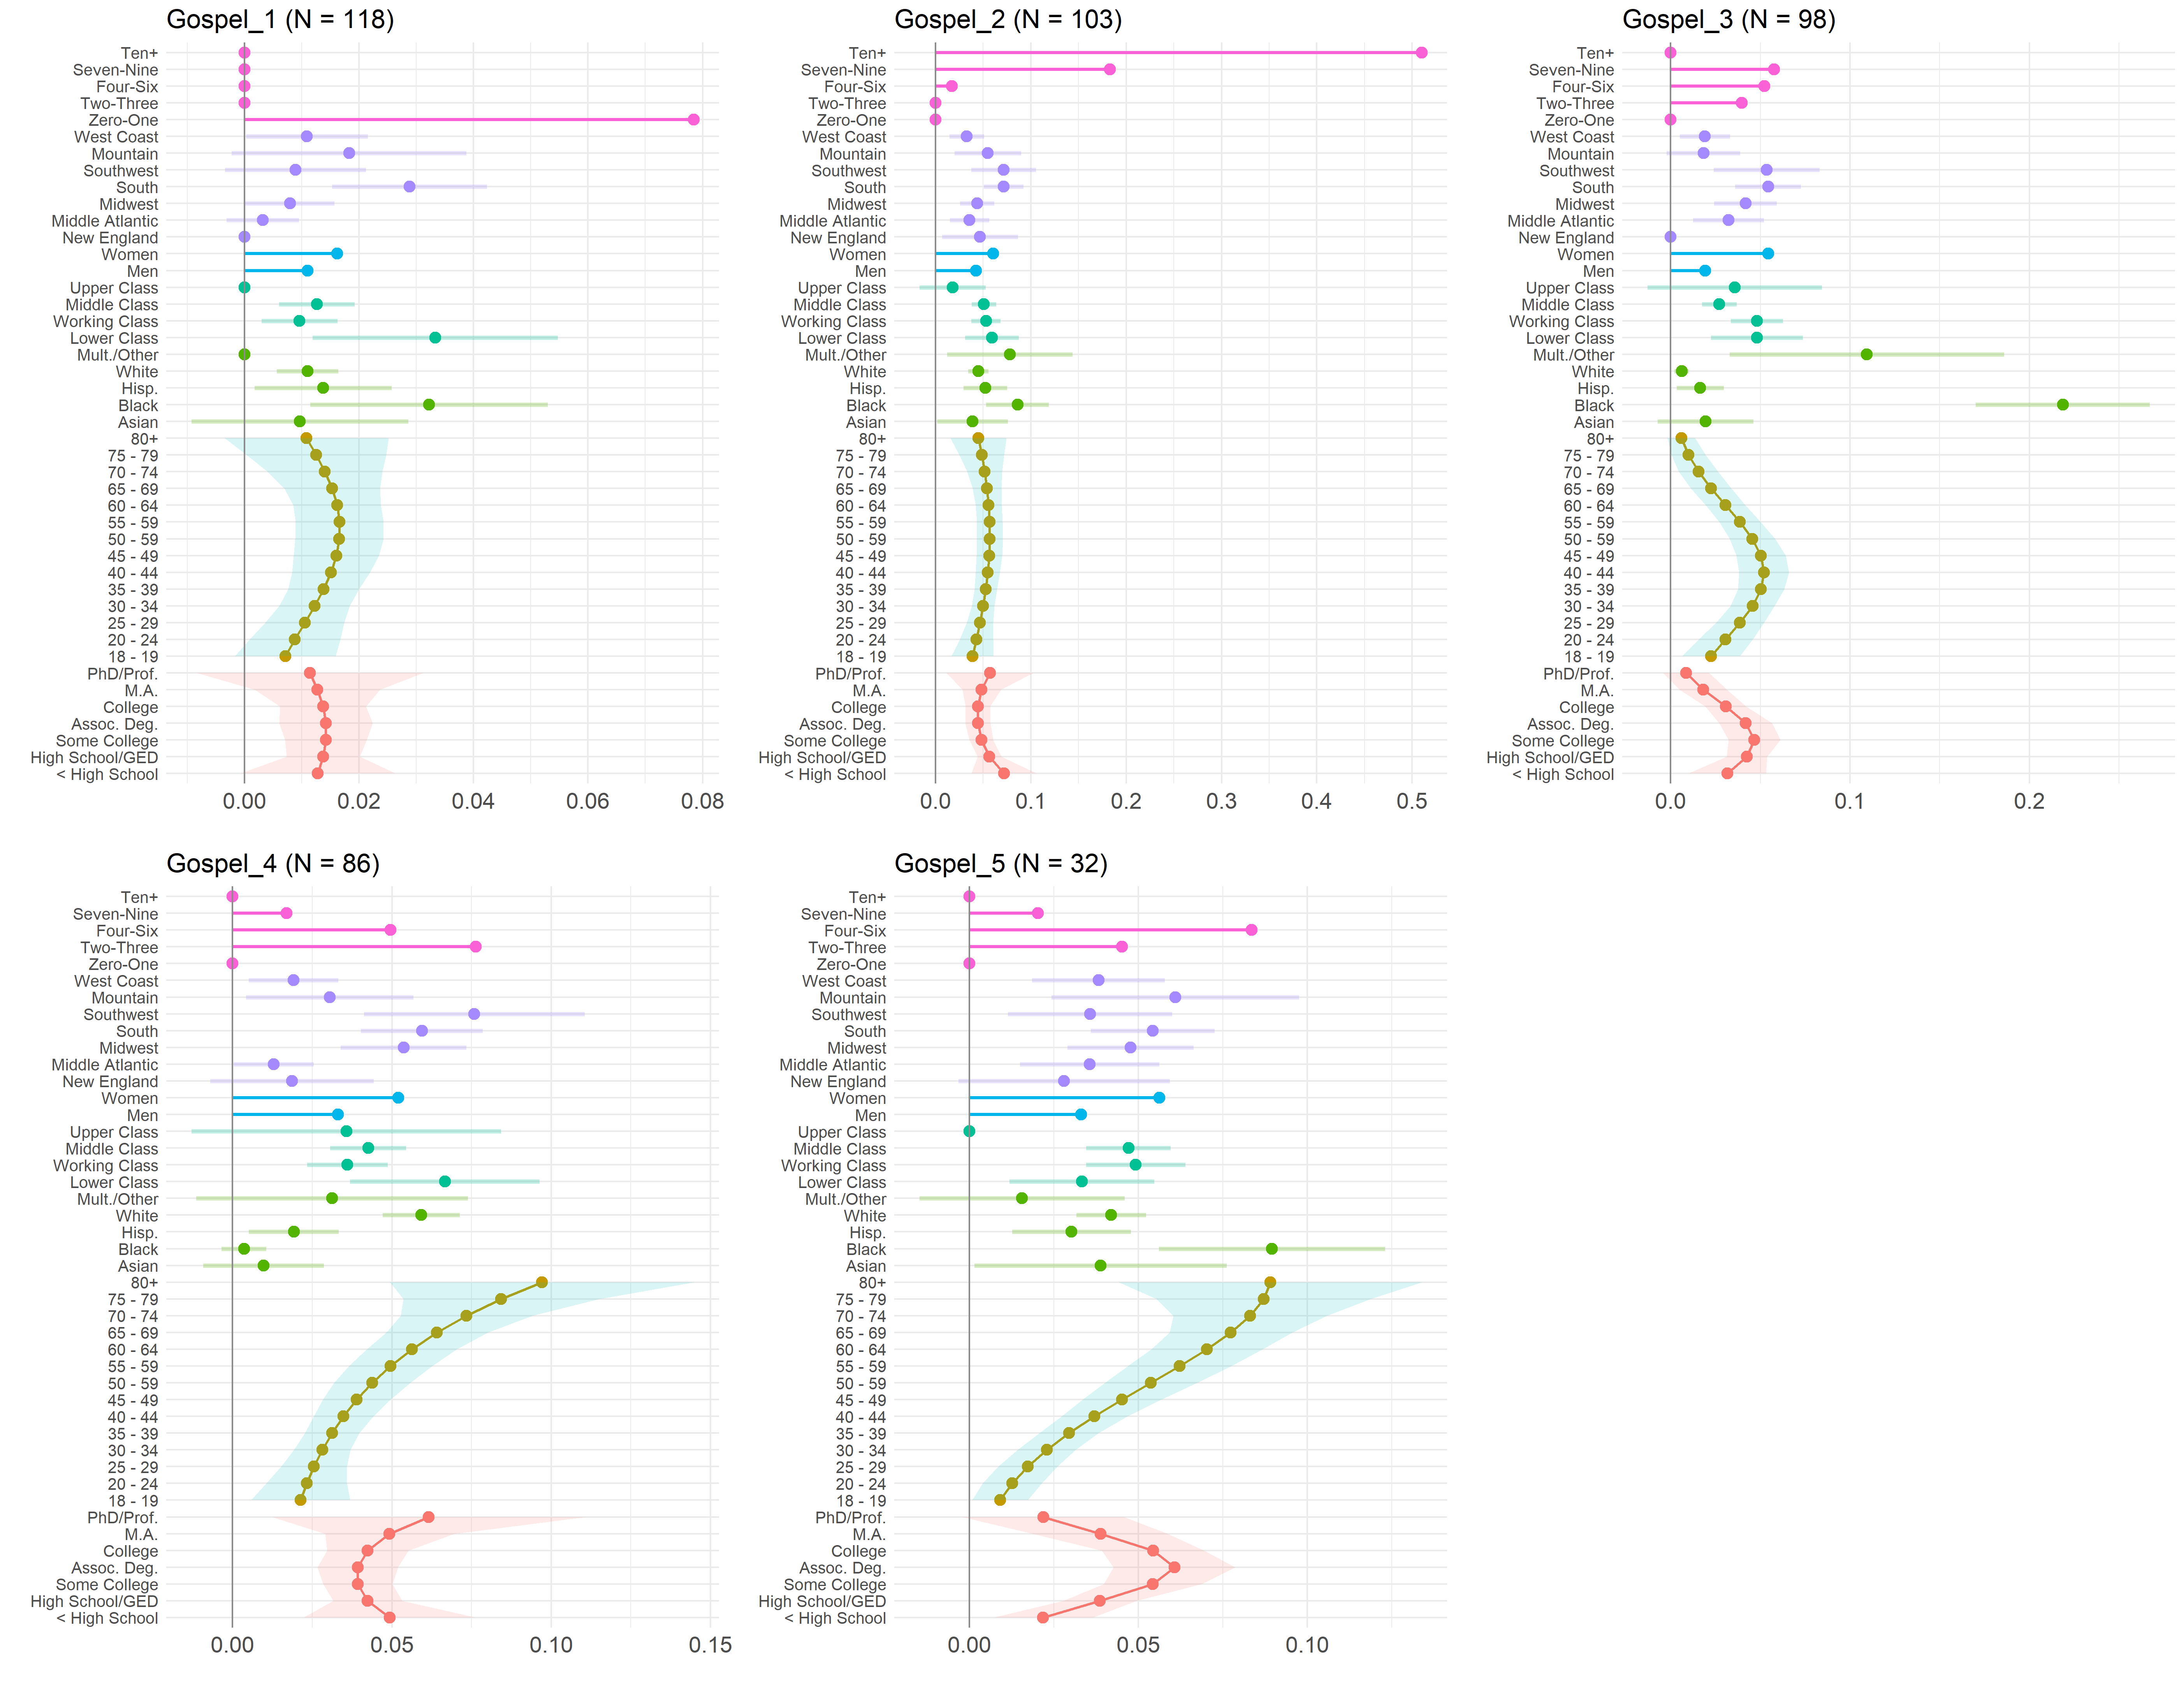
\includegraphics[width=1.0\textwidth]{figs/demog-plots/Gospel.png}
 \caption{}
  \label{fig:gospel}
 \end{figure}

\subsection{Latin/Spanish/Salsa}
Even when macro-genre labels point to styles with some level of presumed audience homogeneity around specific markers (e.g., ethnoracial status), the link micro-genre community approach can discover variations that differ in terms of other social markers. The (already hybrid) macro-genre label ``Latin/Spanish/Salsa'' is a good case in point (see Figure~\ref{fig:latin}). This macro-genre splits into five variations; all are overwhelmingly more likely to be engaged by people who identify as Hispanic (except for 3 which also attract people who identify as multiracial or ``other''). Yet, they differ on key characteristics that cut across ethnic identification. Versions 1, 3, and 4 are more likely to attract young people of middling education, but those who prefer 1 and 3 more likely to combine this engagement with engagement of other genres. The second Latin micro-genre variation, on the other hand, appeals to middle-age people (mainly women) who have more education and identify as middle class. 

 \begin{figure}[ht!]
 \centering
 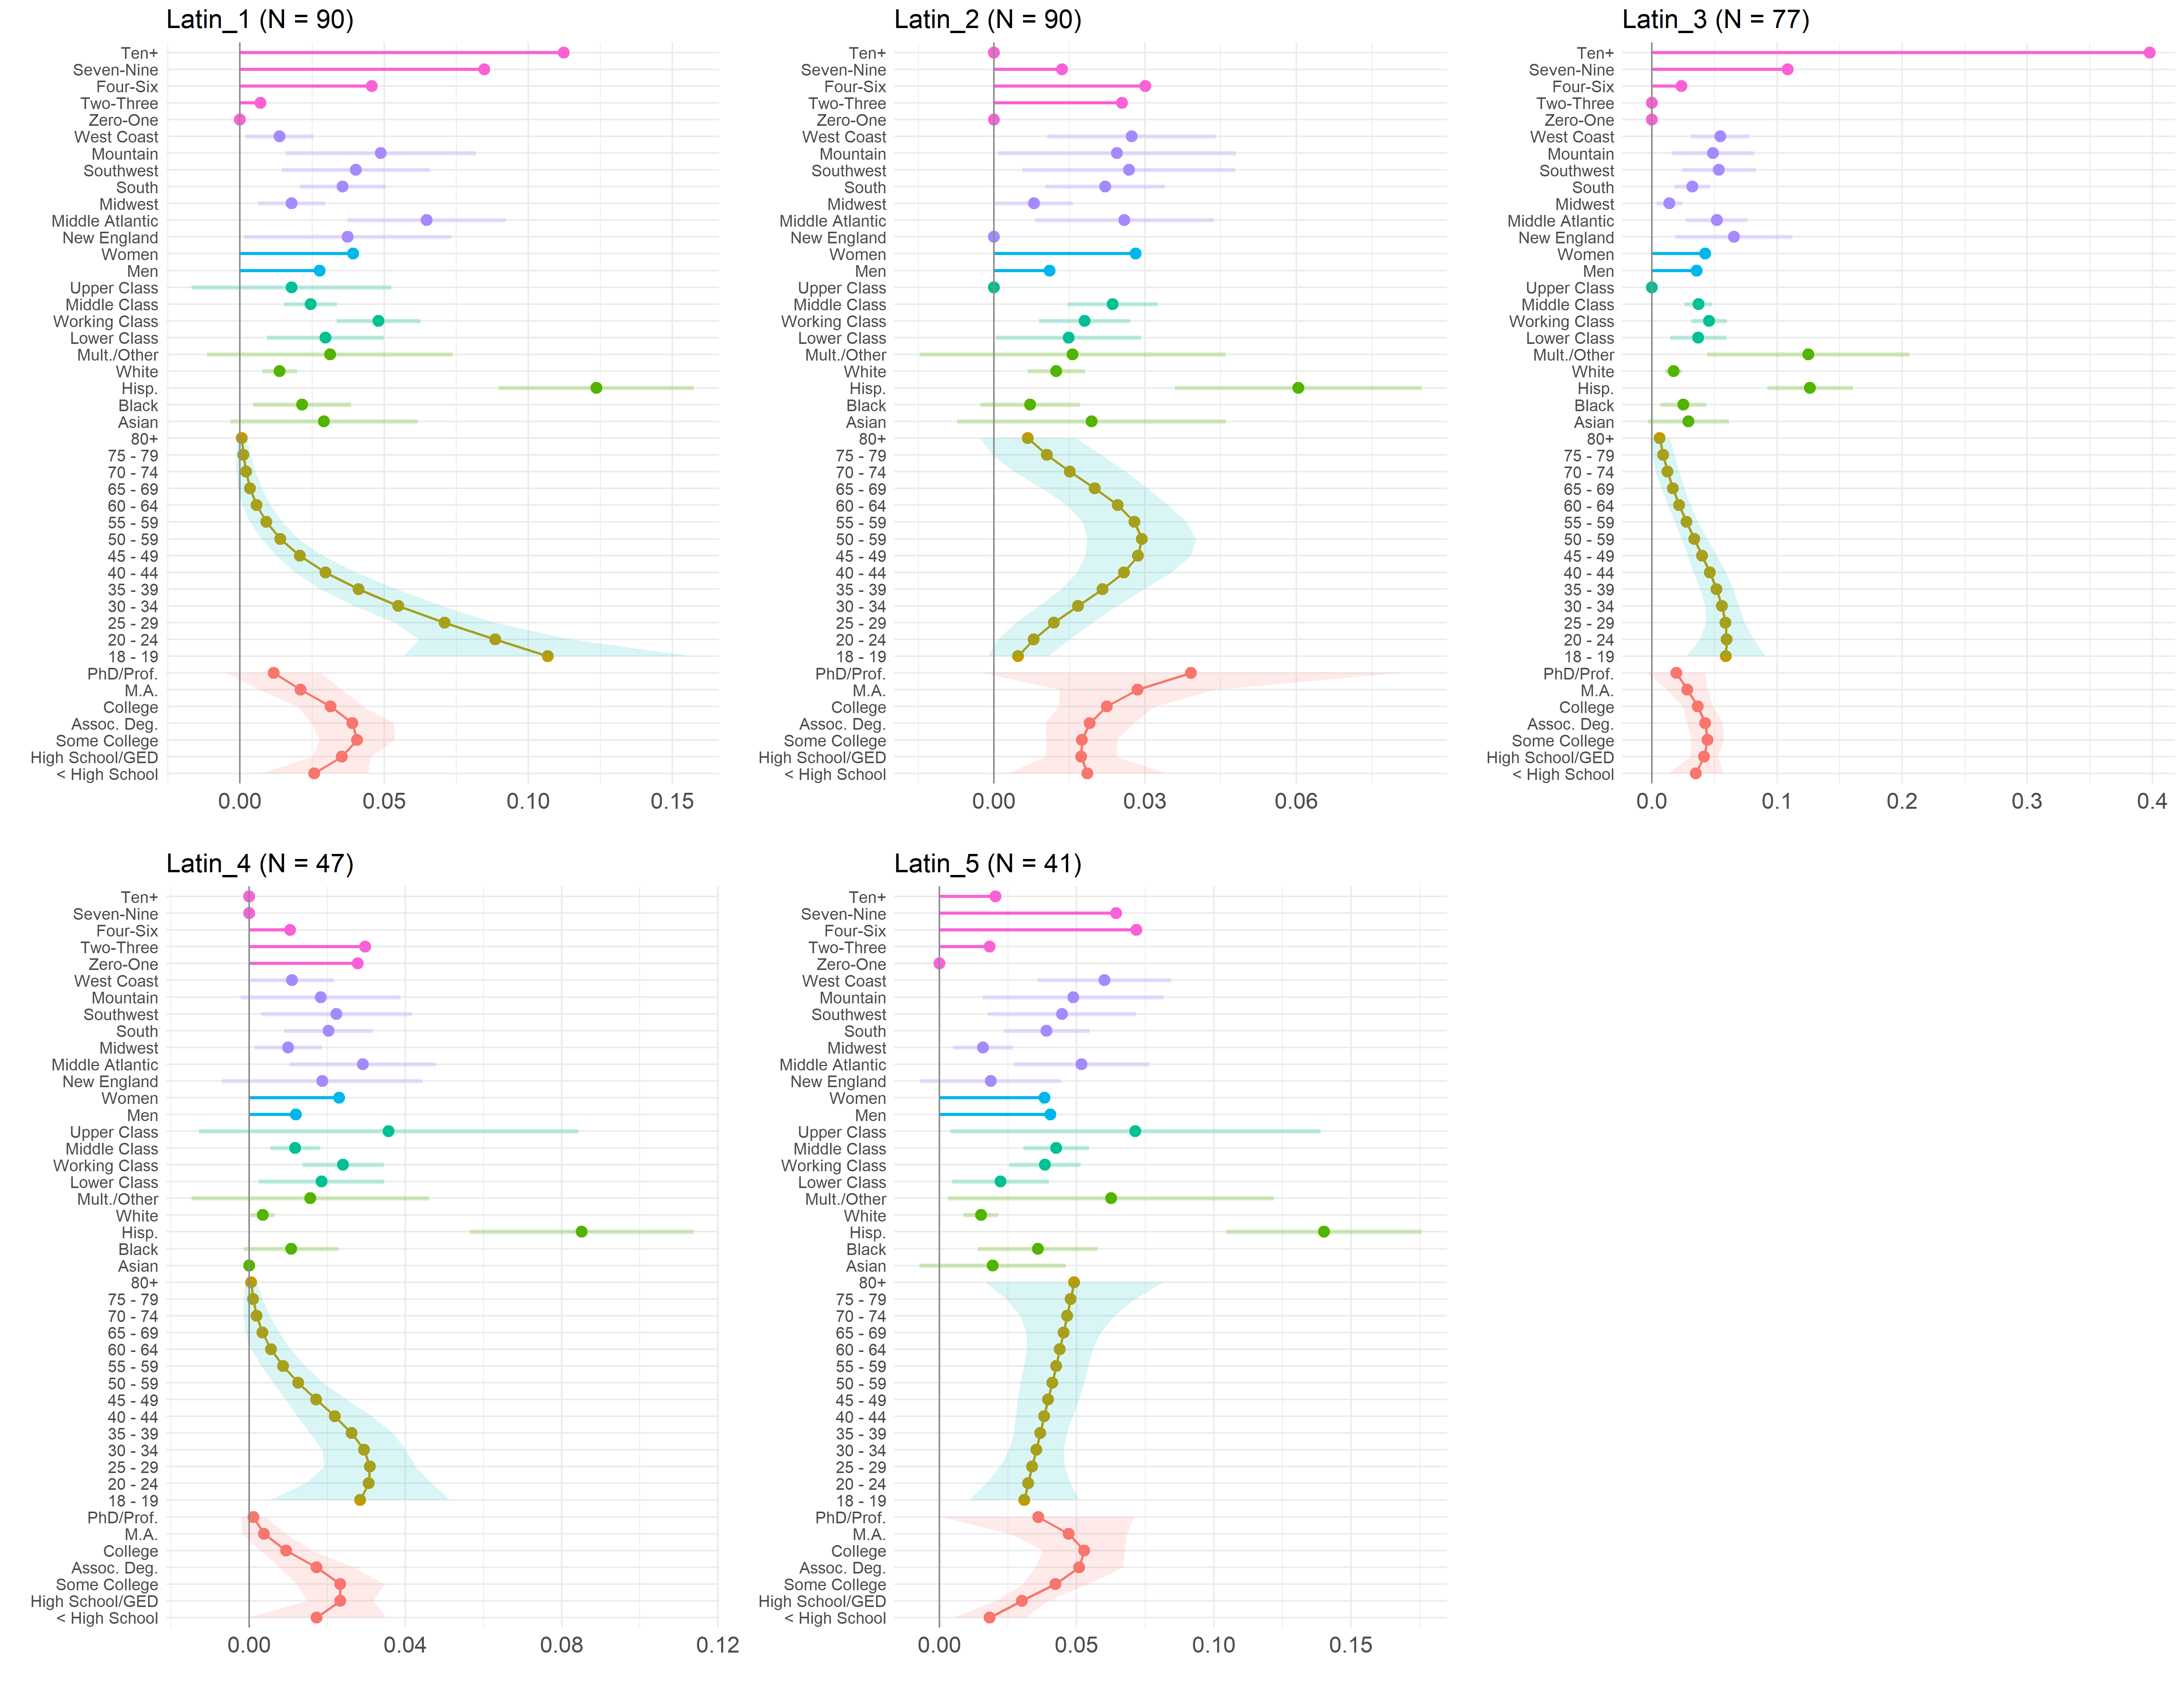
\includegraphics[width=1.0\textwidth]{figs/demog-plots/Latin.png}
 \caption{}
  \label{fig:latin}
 \end{figure}
 
 \subsection{Heavy Metal}
Previous studies in the sociology of taste show that no genre is more polarizing than Heavy Metal. Even the most ``tolerant'' of omnivores have no problem expressing dislike of it. Mass stereotypes of the genre \citep{lizardo_skiles16}, show it to be associated with less educated, ``lower'' or working-class young white men, which accounts for its persistent role as a resource for symbolic boundary drawing, as encoded in the title of Bryson's \citeyearpar{bryson96} classic paper. But in (liking or rejecting) Metal, are Americans affiliating or disaffiliating from a single monolithic thing? As shown in Figure~\ref{fig:metal}, the micro-genre analysis discovers four variations of the ``heavy metal'' micro-genre. These results show support for the idea of ``Heavy Metal'' being one of the most socio-demographically consistent genres, but also show important \textit{generational} variations in its micro-instantiations. On the consistency side, the sociodemographic reality of engagement seems to conform to stereotypical perceptions. Heavy Metal is gendered, racialized, and classed. 

  \begin{figure}[ht!]
     \centering
     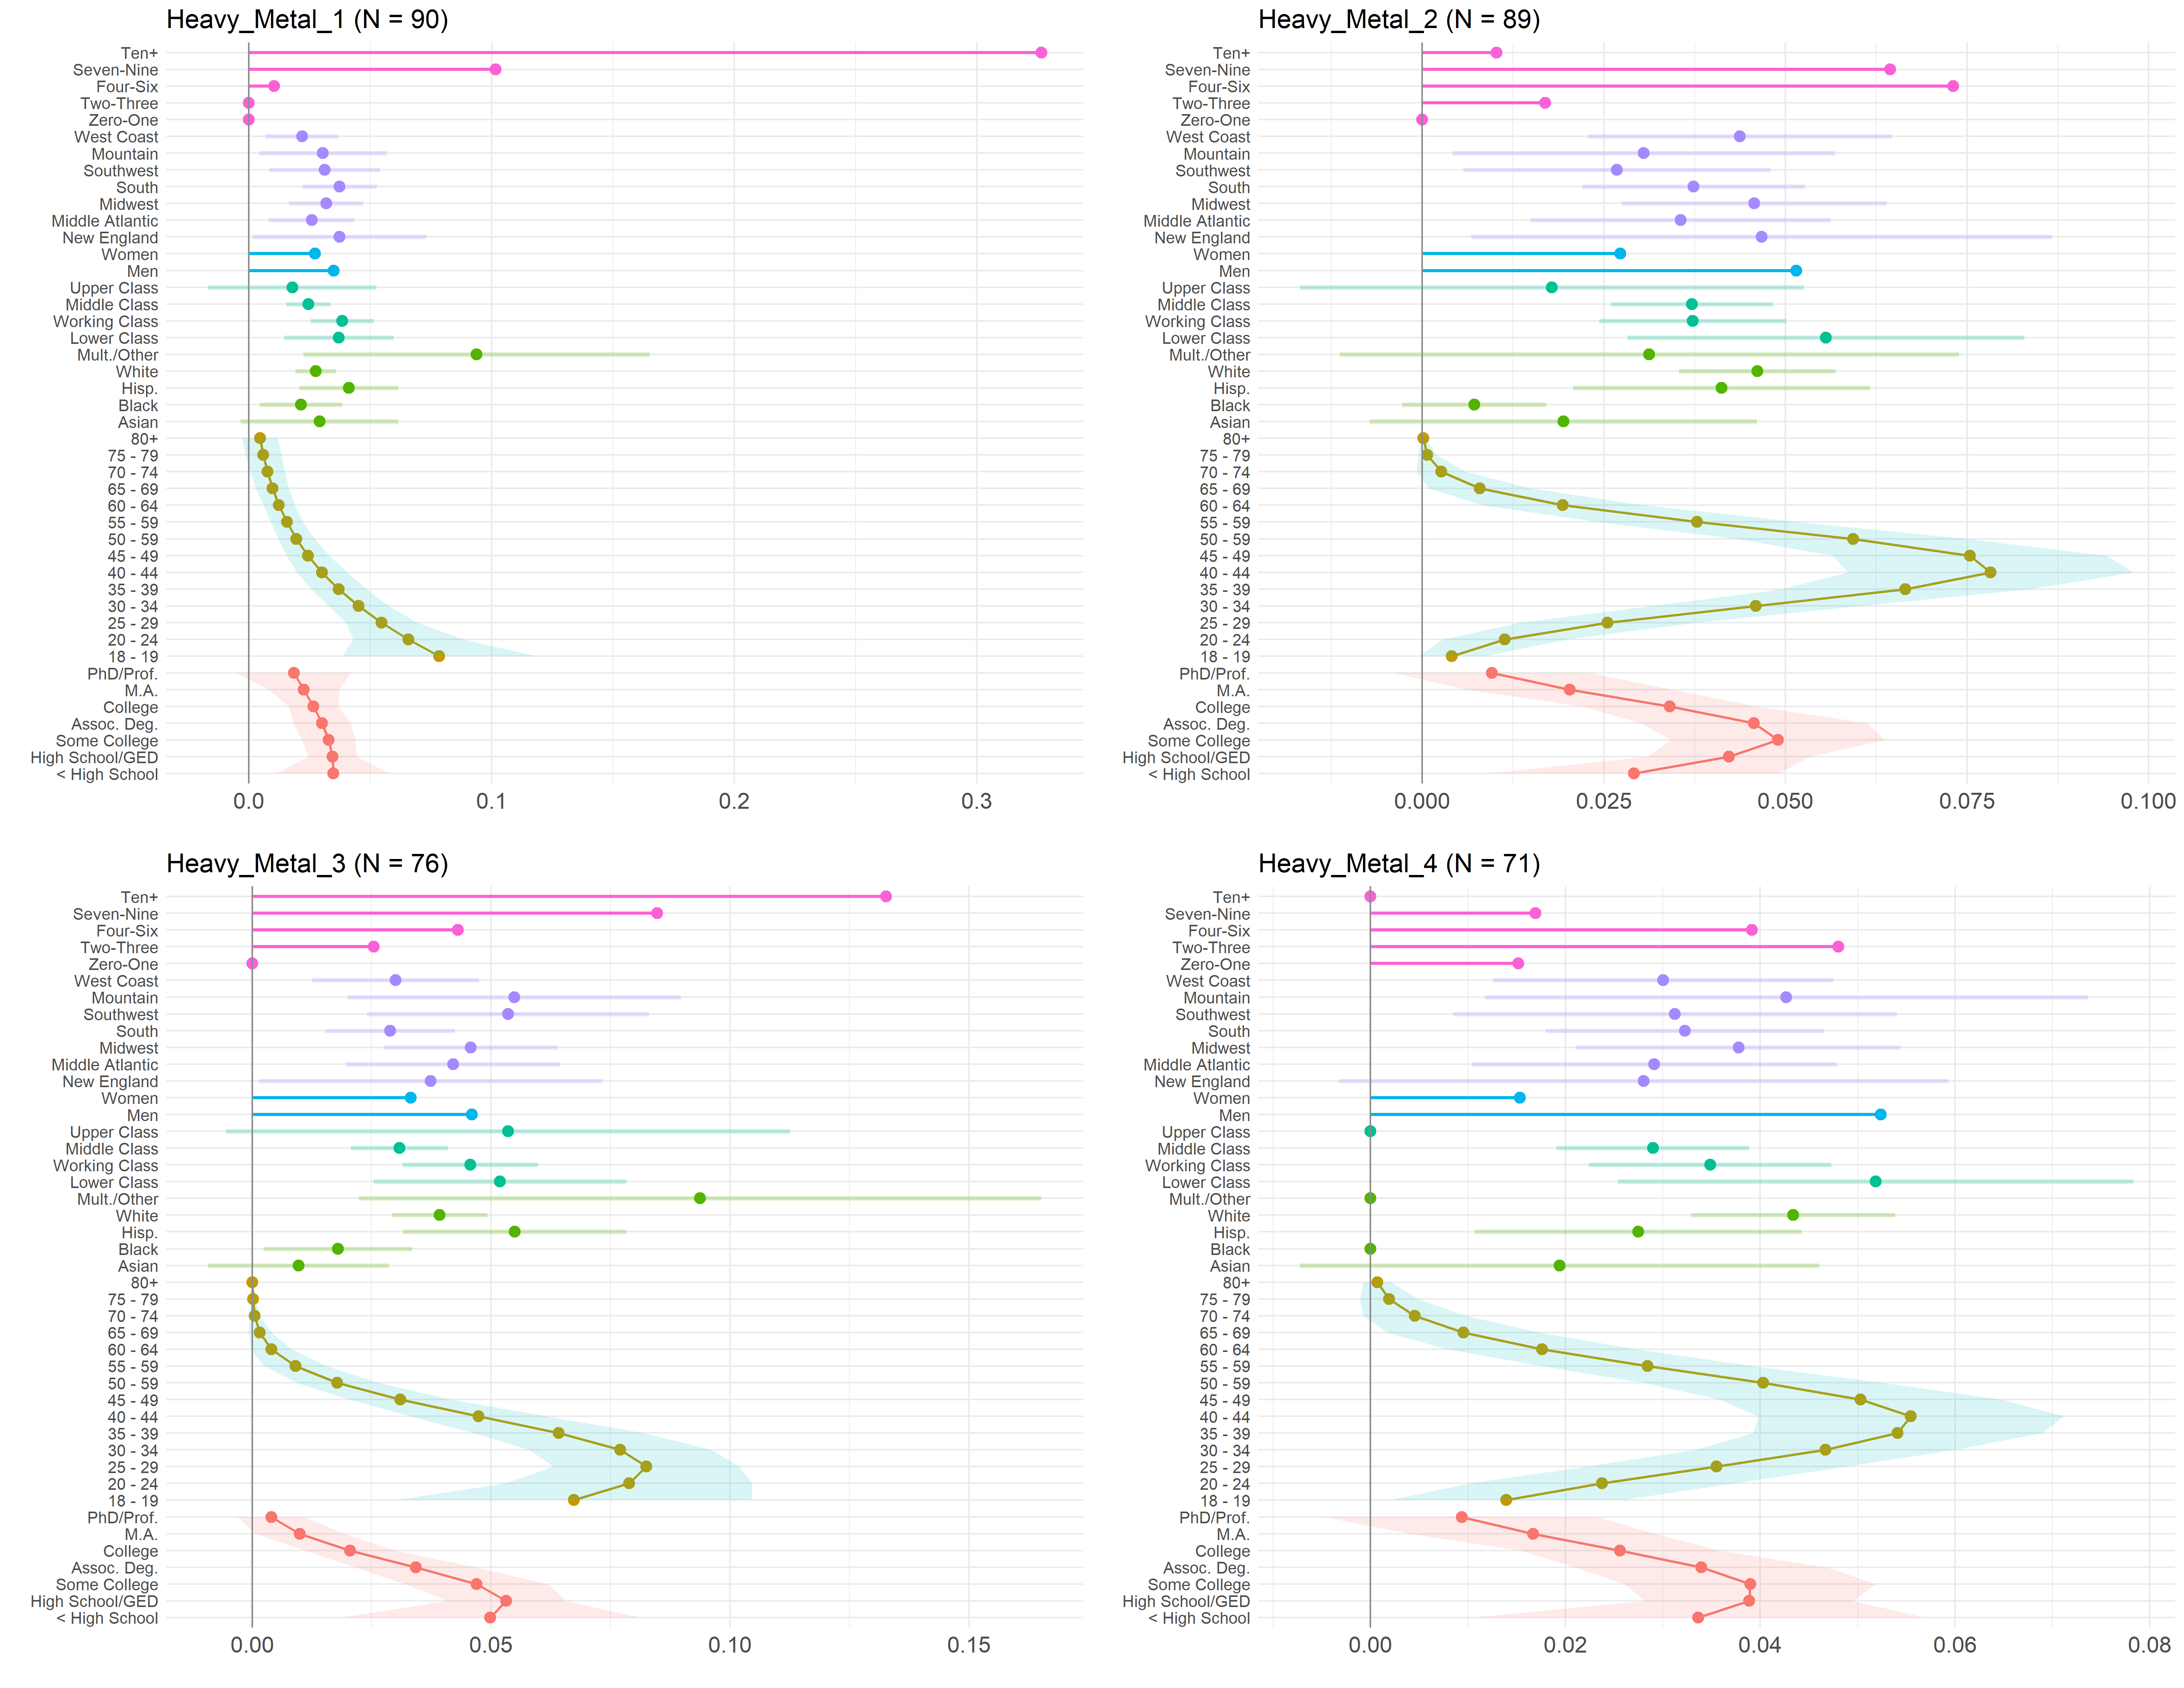
\includegraphics[width=1.0\textwidth]{figs/demog-plots/Heavy_Metal.png}
     \caption{}
  \label{fig:metal}
 \end{figure}
 
Men are more likely to engage all micro-genre variants more than women, consistent with previous work pointing to the strong gendering of the genre \citep{miller2016gender}. The only difference, among the four micro-genres uncovered is the size of the men-to-women disparity. For instance, ``Heavy\_Metal 3" ($N = 75$) is the most tilted toward men, while variations 1 ($N=89$) and 4 ($N=70$) are less so. White respondents are more likely to engage all four micro-genre variations, but so are those who classify themselves as ``multiracial or other," especially for the Metal micro-variation that mixes well with other genres (although the relatively small number of these respondents does not lead to very precise estimates). Surprisingly, for three of the four variations (excepting 4), respondents how identify as Hispanic are statistically more likely to engage the genre than Black respondents. In the same way, for three of the four variations, Metal fans are less likely to have a college degree, although variant 2 ($N = 88$) shows a tilt toward middling (e.g., ``some college'') levels of education. Interestingly, this is also the micro-genre that has the highest concentration of middle-aged adult respondents (e.g., people in their 40s and 50s). The subjective class identification of Metal fans does controvert that projected to them by others; while it is true that some micro-variations are likely to feature people who identify as either lower or working class, they are likely to contain statistically indistinguishable proportions of people who identify as middle class. 
 
\subsection{Classic Rock/Oldies}
Perhaps the test case for the misleading nature of the macro-genre label approach are composite or vague labels like ``Classic Rock/Oldies.'' The suspicion is that such a vague designation hides a wide variety of more focused and perhaps stylistically and demographically disjoint micro-genres. The link-community approach produces results consistent with this claim. This macro-genre label (the most ``popular'' in terms of audience size in the original data) is also the one that splits into the largest number (thirteen) of micro-genres, shown in Figures~\ref{fig:Class-Rock1}, and~\ref{fig:Class-Rock2}. These vary substantially in terms of all the sociodemographic indicators considered. 

\begin{figure}[ht!]
    \centering
     \begin{subfigure}[b]{0.8\textwidth}
        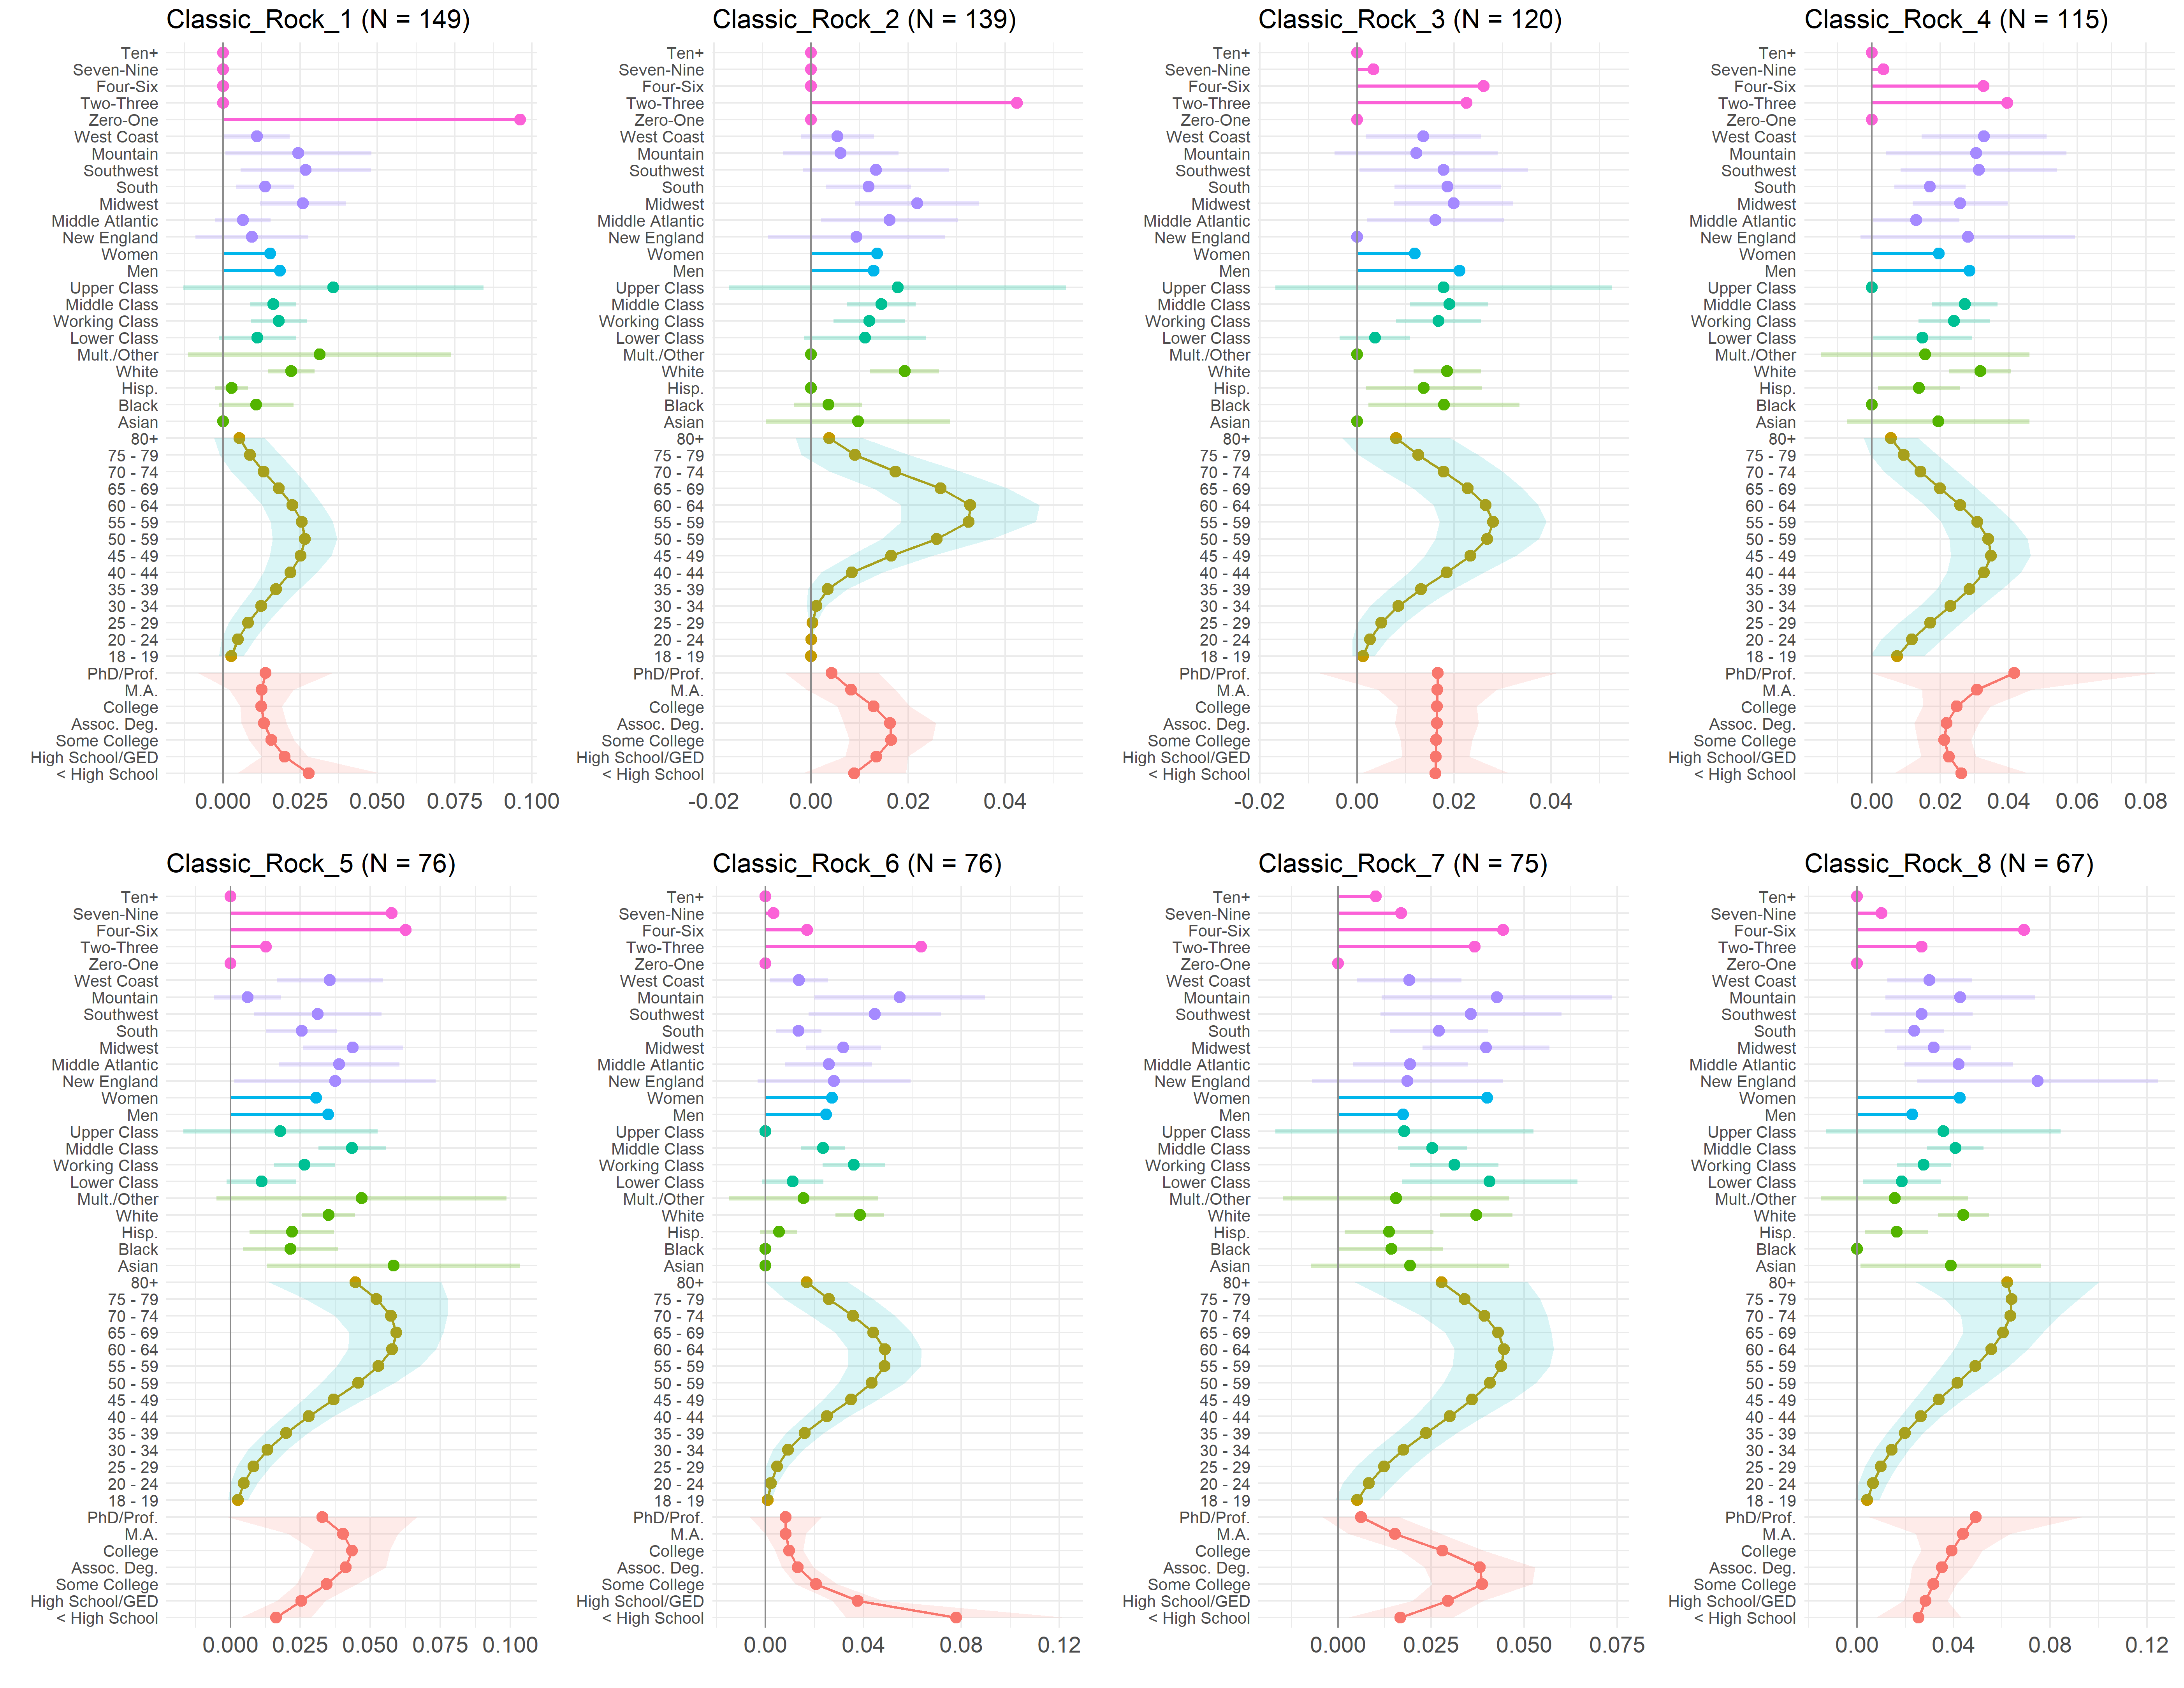
\includegraphics[width=1.0\textwidth]{figs/demog-plots/Classic_Rock1.png}
        \caption{}
        \label{fig:Class-Rock1}
    \end{subfigure} 
     \begin{subfigure}[b]{0.8\textwidth}
        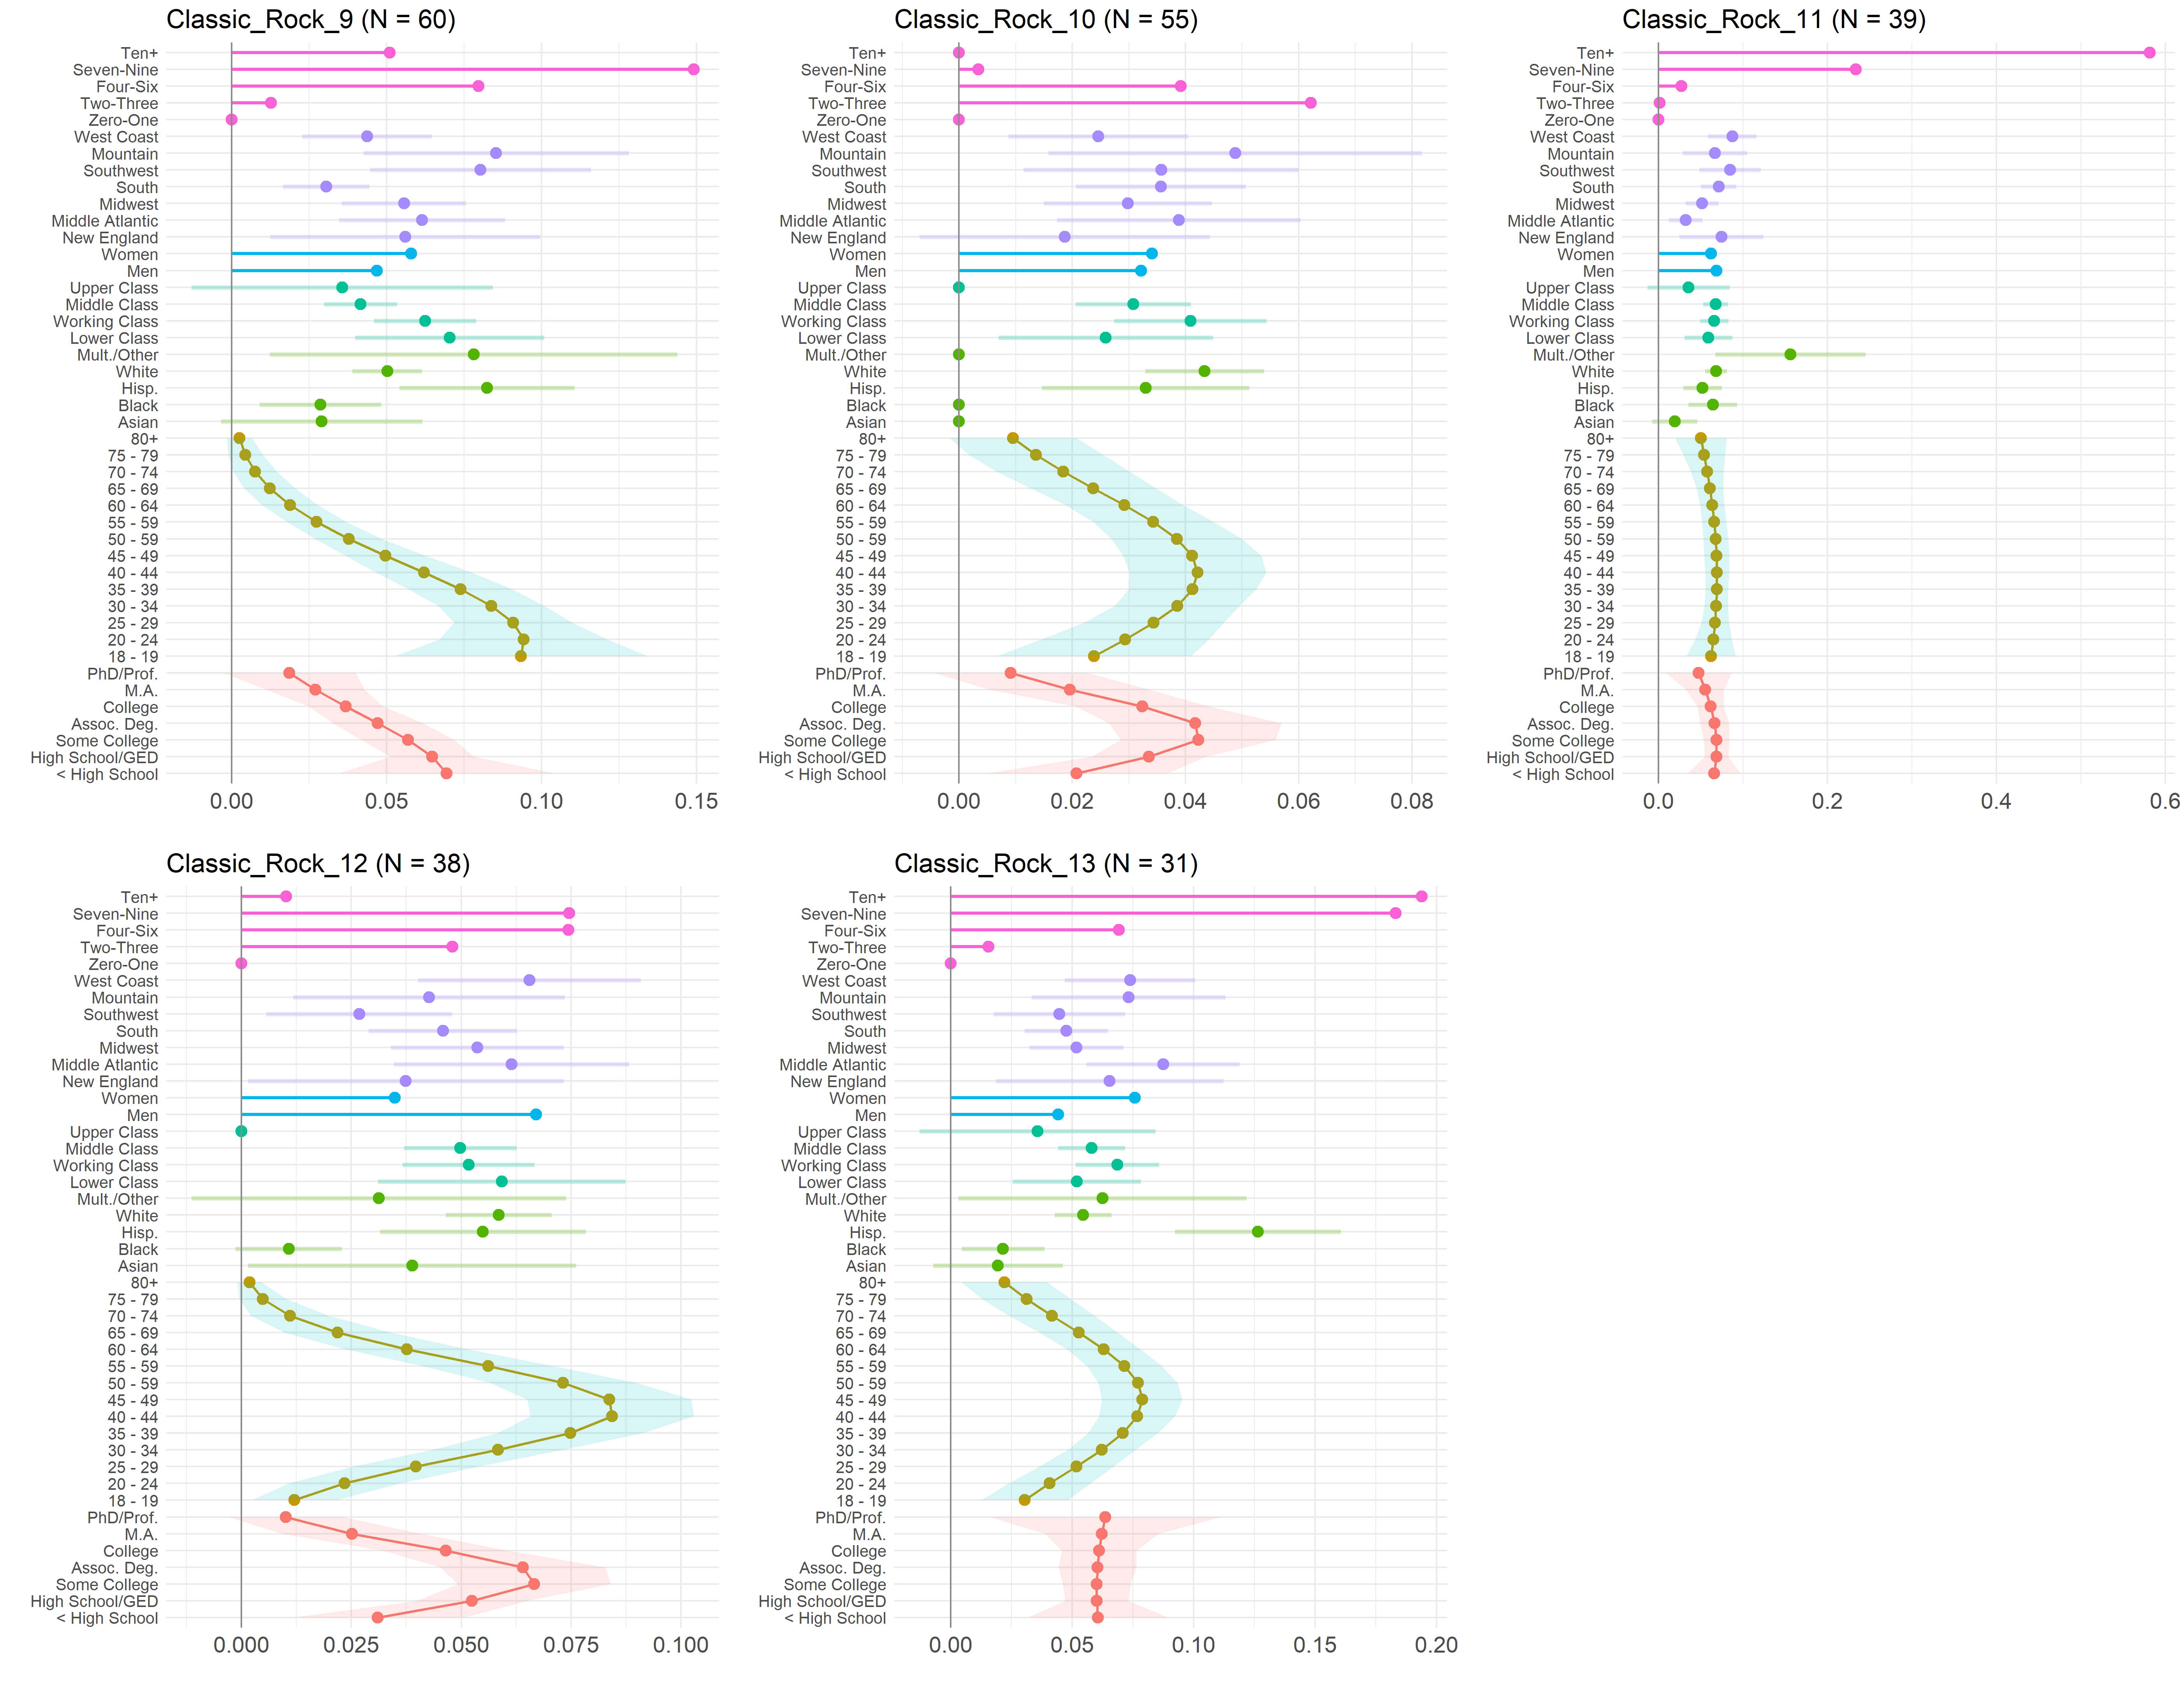
\includegraphics[width=1.0\textwidth]{figs/demog-plots/Classic_Rock2.png}
        \caption{}
        \label{fig:Class-Rock2}
    \end{subfigure}
     \caption{}
  \label{fig:Class-Rock}
 \end{figure}
 
The largest community (version 1, $N = 149$) depicts the Classic Rock univore; a middle-aged white person who resides in the Midwest, Southwest or Mountain West with less than a high-school education. The second-largest Classic Rock micro-genre ($N = 139$ is a lot like the first, except that the tilt to older respondents is much stronger as is concentration among respondents who either finished high school or received some college education. But perhaps the prototypical Classic Rock micro-genre is version 6 ($N = 76$), appealing to older respondents very much likely to identify as both white and working class, with relatively low education, who reside in the Mountain and Southwest region. 

Some of the smaller micro-genre communities controvert the usual expectations as to who is the typical Classic Rock/Oldies fan \citep{lizardo_skiles16}. For instance, people who engage variation 9 ($N = 60$) are of low education (which is expected), but they are also likely to be very young, working or middle class-identified Hispanics with less than a high school education and live in the Southwest. Version 10 ($N = 55$ is a lot like this last one, but concentrates among respondents with some college attainment; yet another variant of this micro-genre (version 13, $N = 31$) tilts toward middle-aged Hispanic-identified women who live on either coast.\footnote{Perhaps these last set of respondents understand ``Classic Rock'' to include such long existing American genres as ``Tex-Mex.''} There is even a version of Classic Rock that contravenes socioeconomic, gender, and regional expectations, appealing to middle-class, highly educated women who identify as white and live in New England (version 8, $N = 32$). 

\subsection{Pop/Top 40}
As shown in Figure~\ref{fig:Pop}, landscape of the very vague macro-genre label ``Pop/Top 40,'' presents as variegated a landscape as that presented by Classic Rock, with ten micro-genre versions. There are consistent (and expected) patterns. In terms of age distribution, Pop micro-genres communities tilt toward the very young (3, 5, and 10, $N=104$, $N=95$, and $N=17$, respectively) or toward young adults (1, 2, $N=143$ and $N=126$). The rest are either age-neutral (7, 8, 9, $N=64$, $N=43$, and $N=30$, respectively) and only two  (4, 6, $N=102$, $N=71$) tilt toward or are preferred by people in their 40s and 50s. None concentrate among older respondents. The very young pop micro-genres communities are differentiated by class: Version 3 is low education, working class, while version 5 is college-educated and middle class. Version 10 is differentiated by gender and race, attracting mainly young nonwhite women. Versions 3, 7, and 8 are pop micro-genres that combine well with others at the level of people's repertoire (their audience tend to be omnivorous), while version 1 reveals a classic pop univore. 
 
  \begin{figure}[ht!]
      \centering
     \begin{subfigure}[b]{0.8\textwidth}
        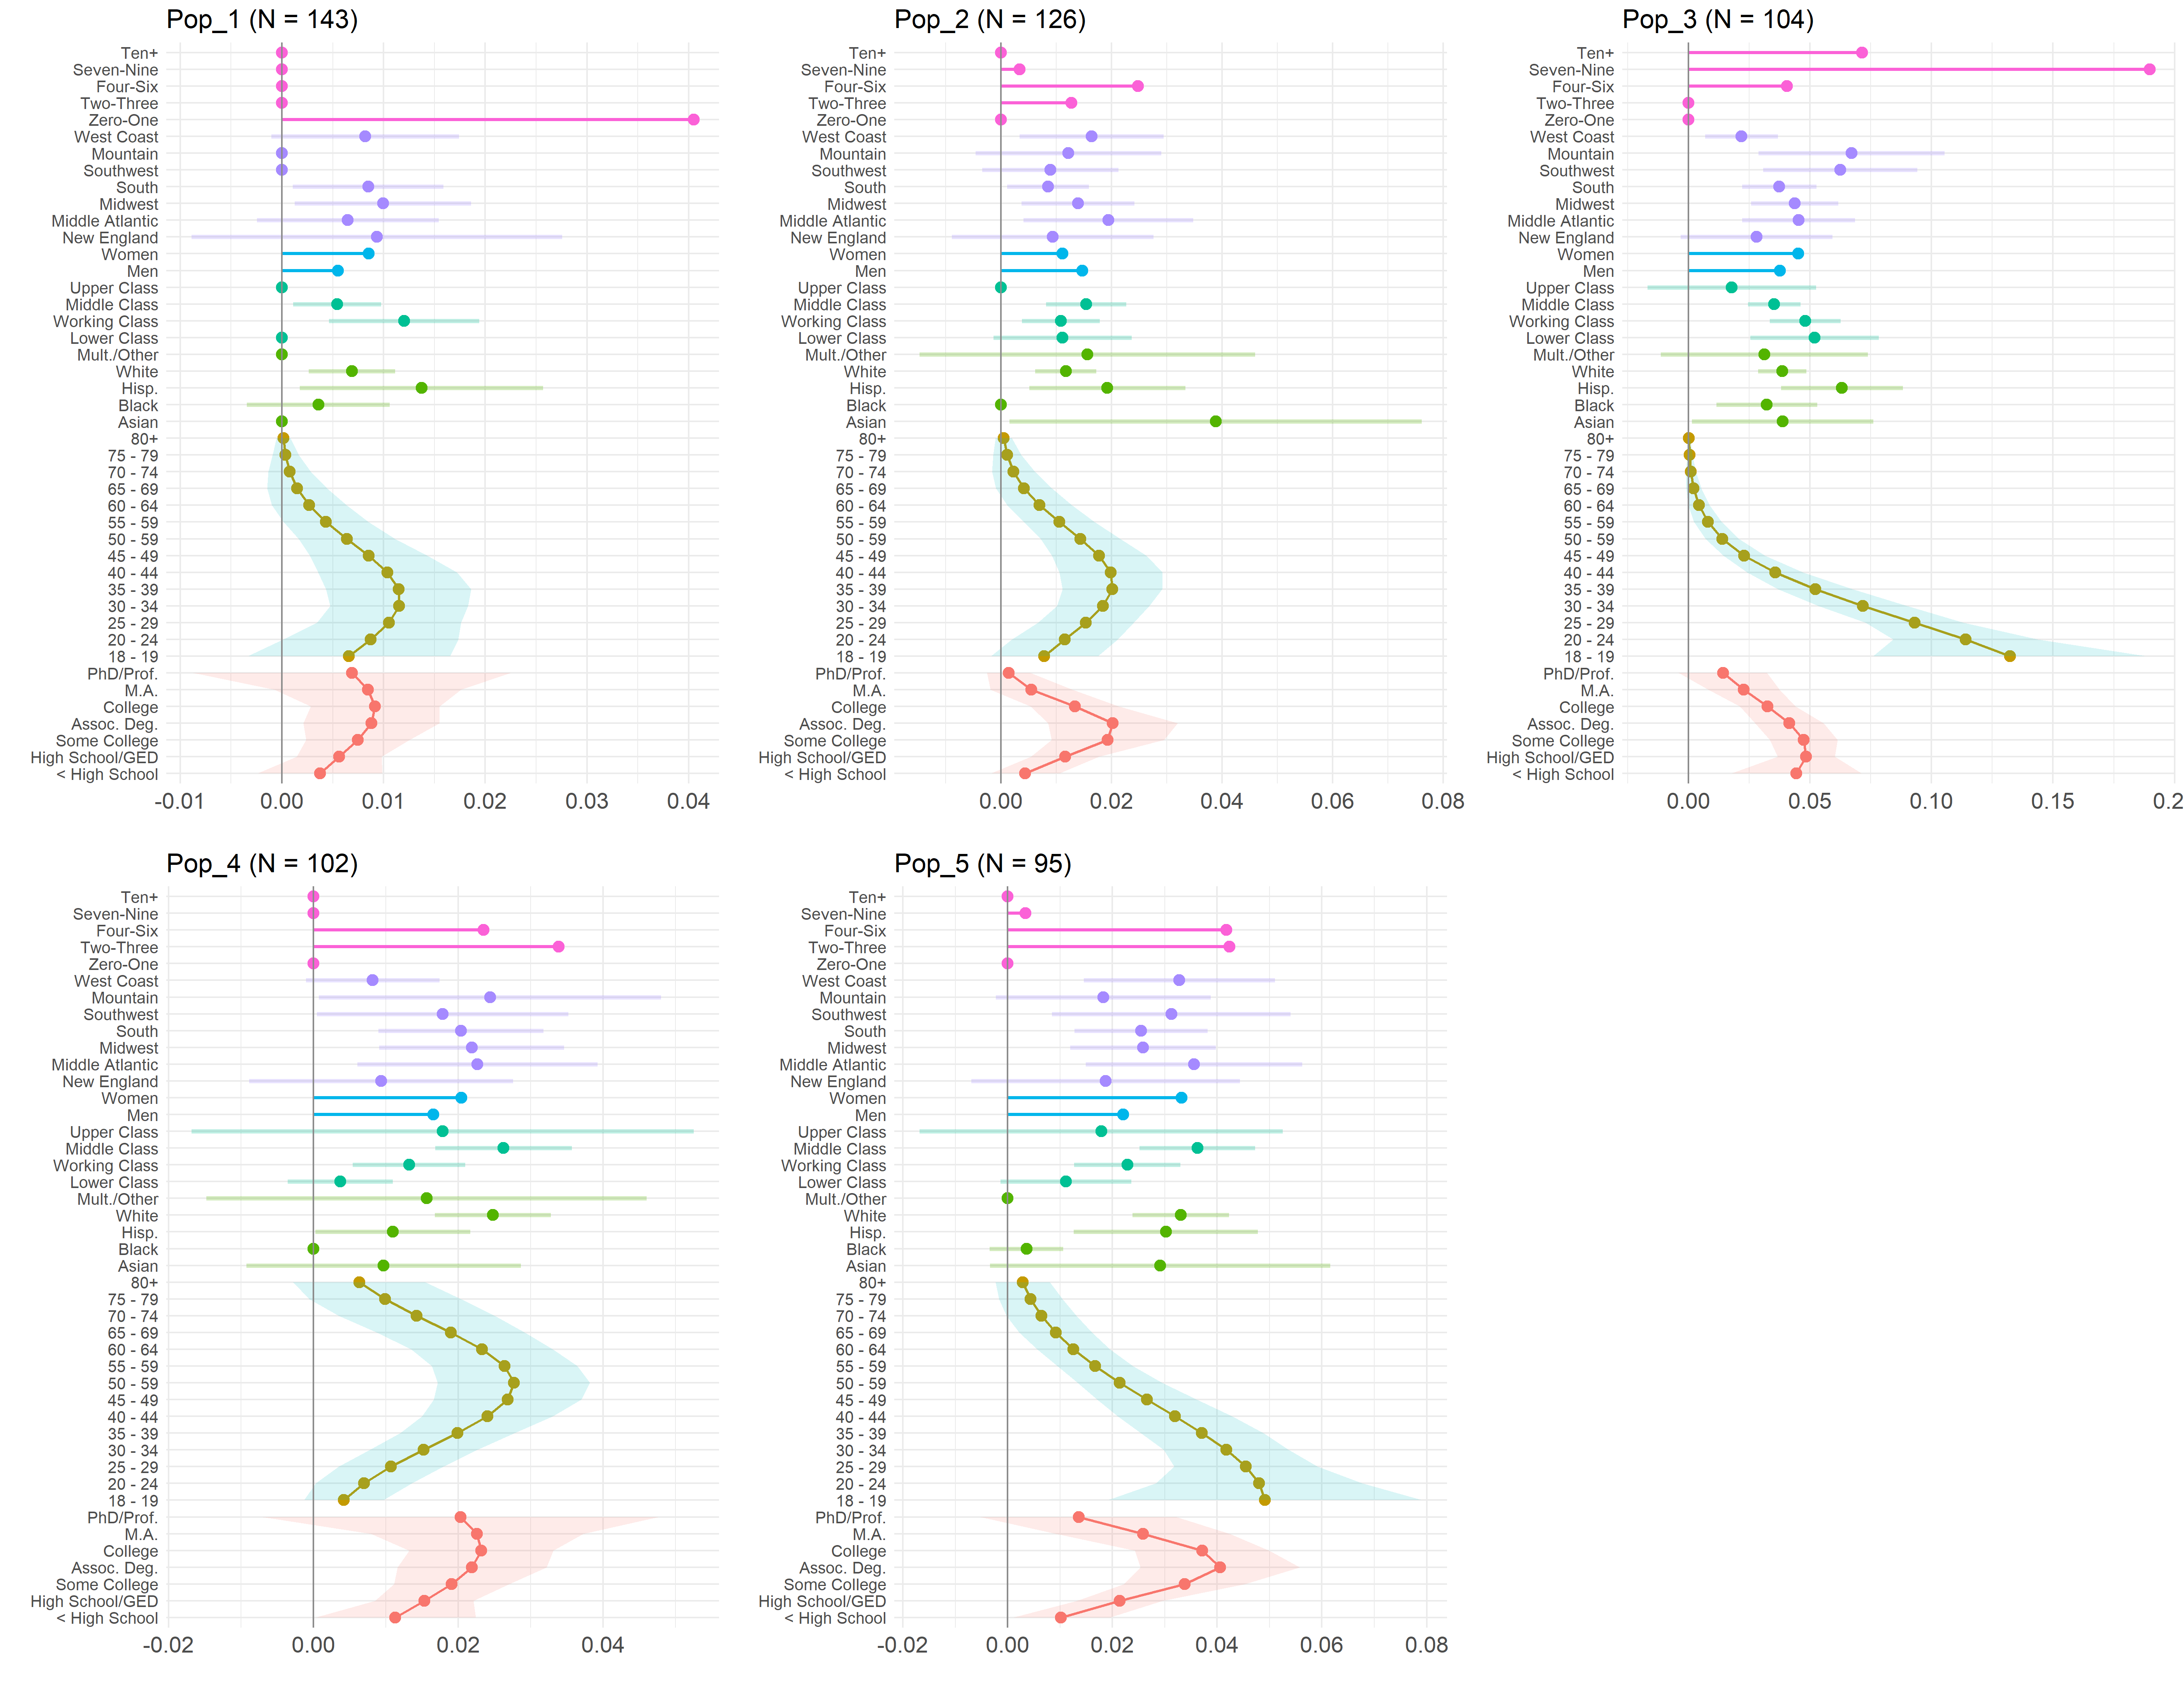
\includegraphics[width=1.0\textwidth]{figs/demog-plots/Pop1.png}
        \caption{}
        \label{fig:Pop1}
    \end{subfigure} 
     \begin{subfigure}[b]{0.8\textwidth}
        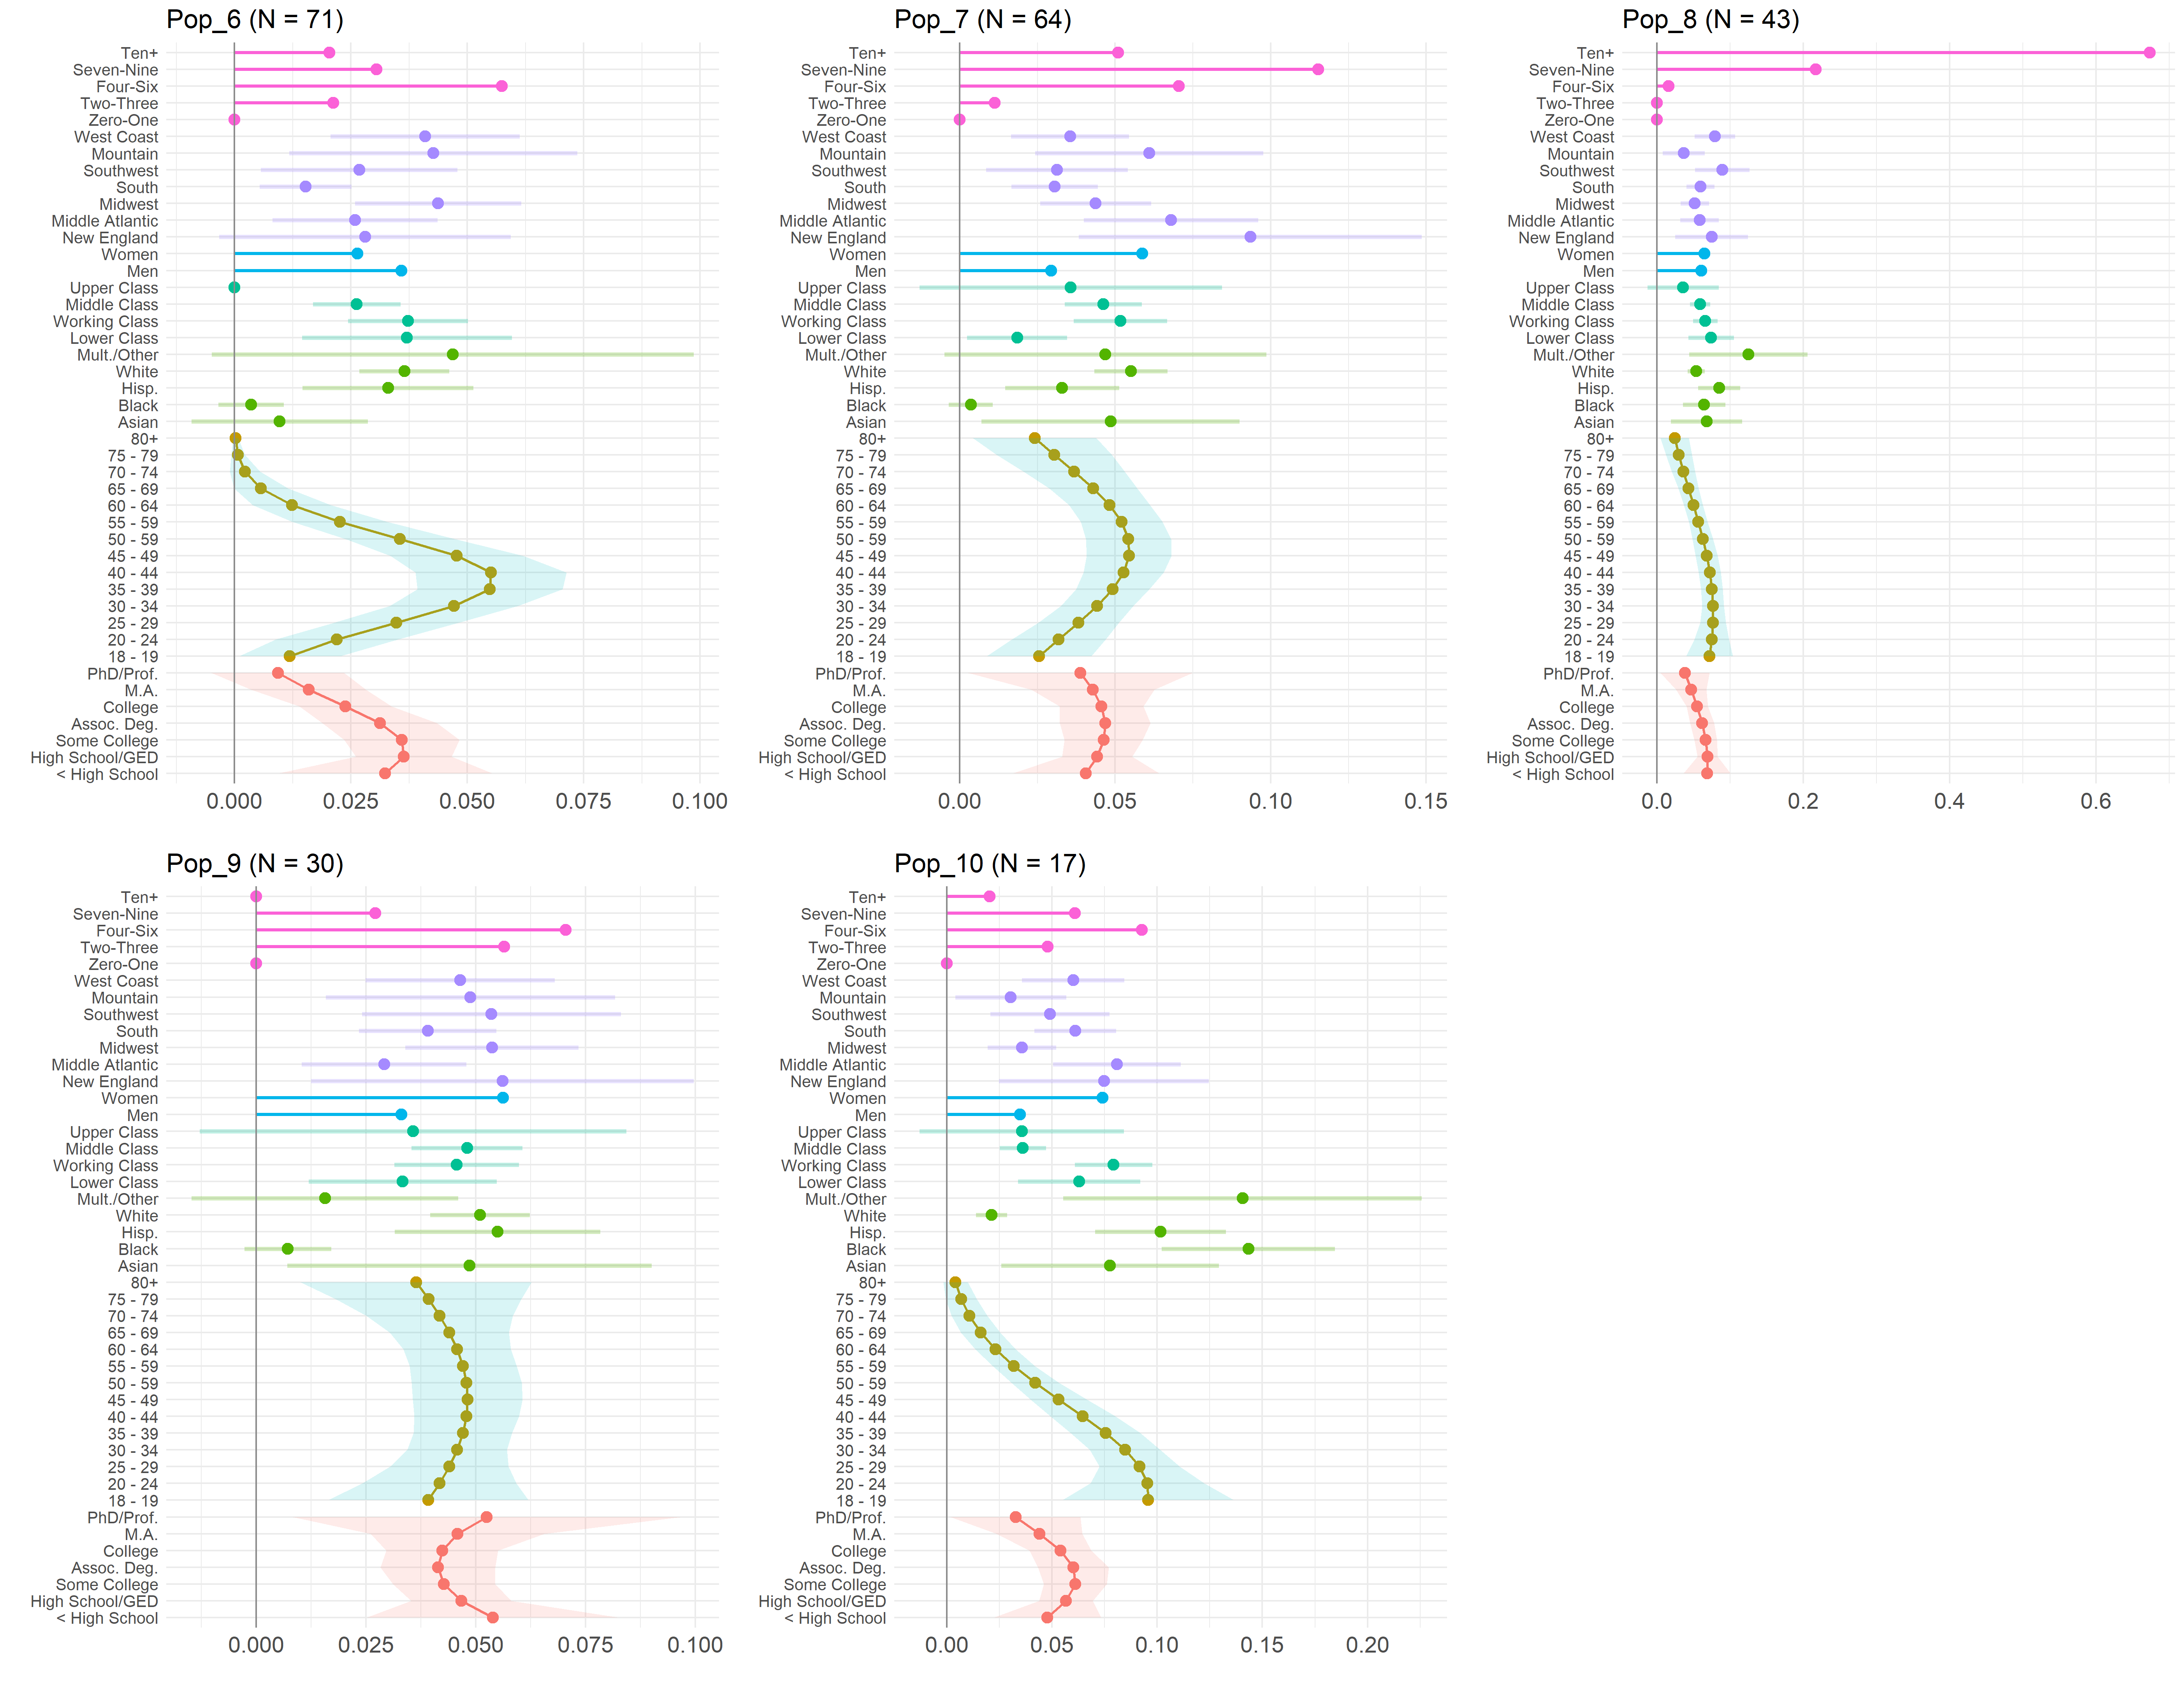
\includegraphics[width=1.0\textwidth]{figs/demog-plots/Pop2.png}
        \caption{}
        \label{fig:Pop2}
    \end{subfigure}
     \caption{}
  \label{fig:Pop}
 \end{figure}
 
\subsection{Country}
The macro-genre label of ``country music'' has always been one suspected of hiding untold levels of micro-genre heterogeneity. This is not only the case style, but also sociodemographics, generations and even politics \citep{rossman2004elites}. As shown in Figure~\ref{fig:Country}, the micro-genres discovered by the cluster analysis agree with this take. First, the analysis reveals ten distinct macro-genres within the larger vague label. Within these, there is strong generational differentiation across different versions of ``country." Five appeal mainly to older audiences (1, 2, 4, 6, 8, $N=123$, $N=115$, $N=87$, $N=70$, and $N=58$, respectively), two tilting toward younger fans (3 and 7, $N=110$ and $N=61$), and two engaging middle-aged people (5 and 10, $N=70$ and $N=49$). Micro-genre 1 recovers the prototypical ``country univore." Fans of these micro-genre are largely white, shun the upper-class label, do not have a college degree, and engage only this micro-genre to the exclusion of others. Version 3, by way of contrast, is the obligatory micro-genre that mixes indiscriminately with other genres. Country micro-genres attracting older respondents exhibit class differentiation, with versions 1, 2, and 6 attracting respondents with less than a college education, and versions 4 and 8 reversing this pattern; the great bulk of fans of country version 4 identify as middle class making this micro-genre distinctive in that respect. 

  \begin{figure}[ht!]
    \centering
     \begin{subfigure}[b]{0.8\textwidth}
        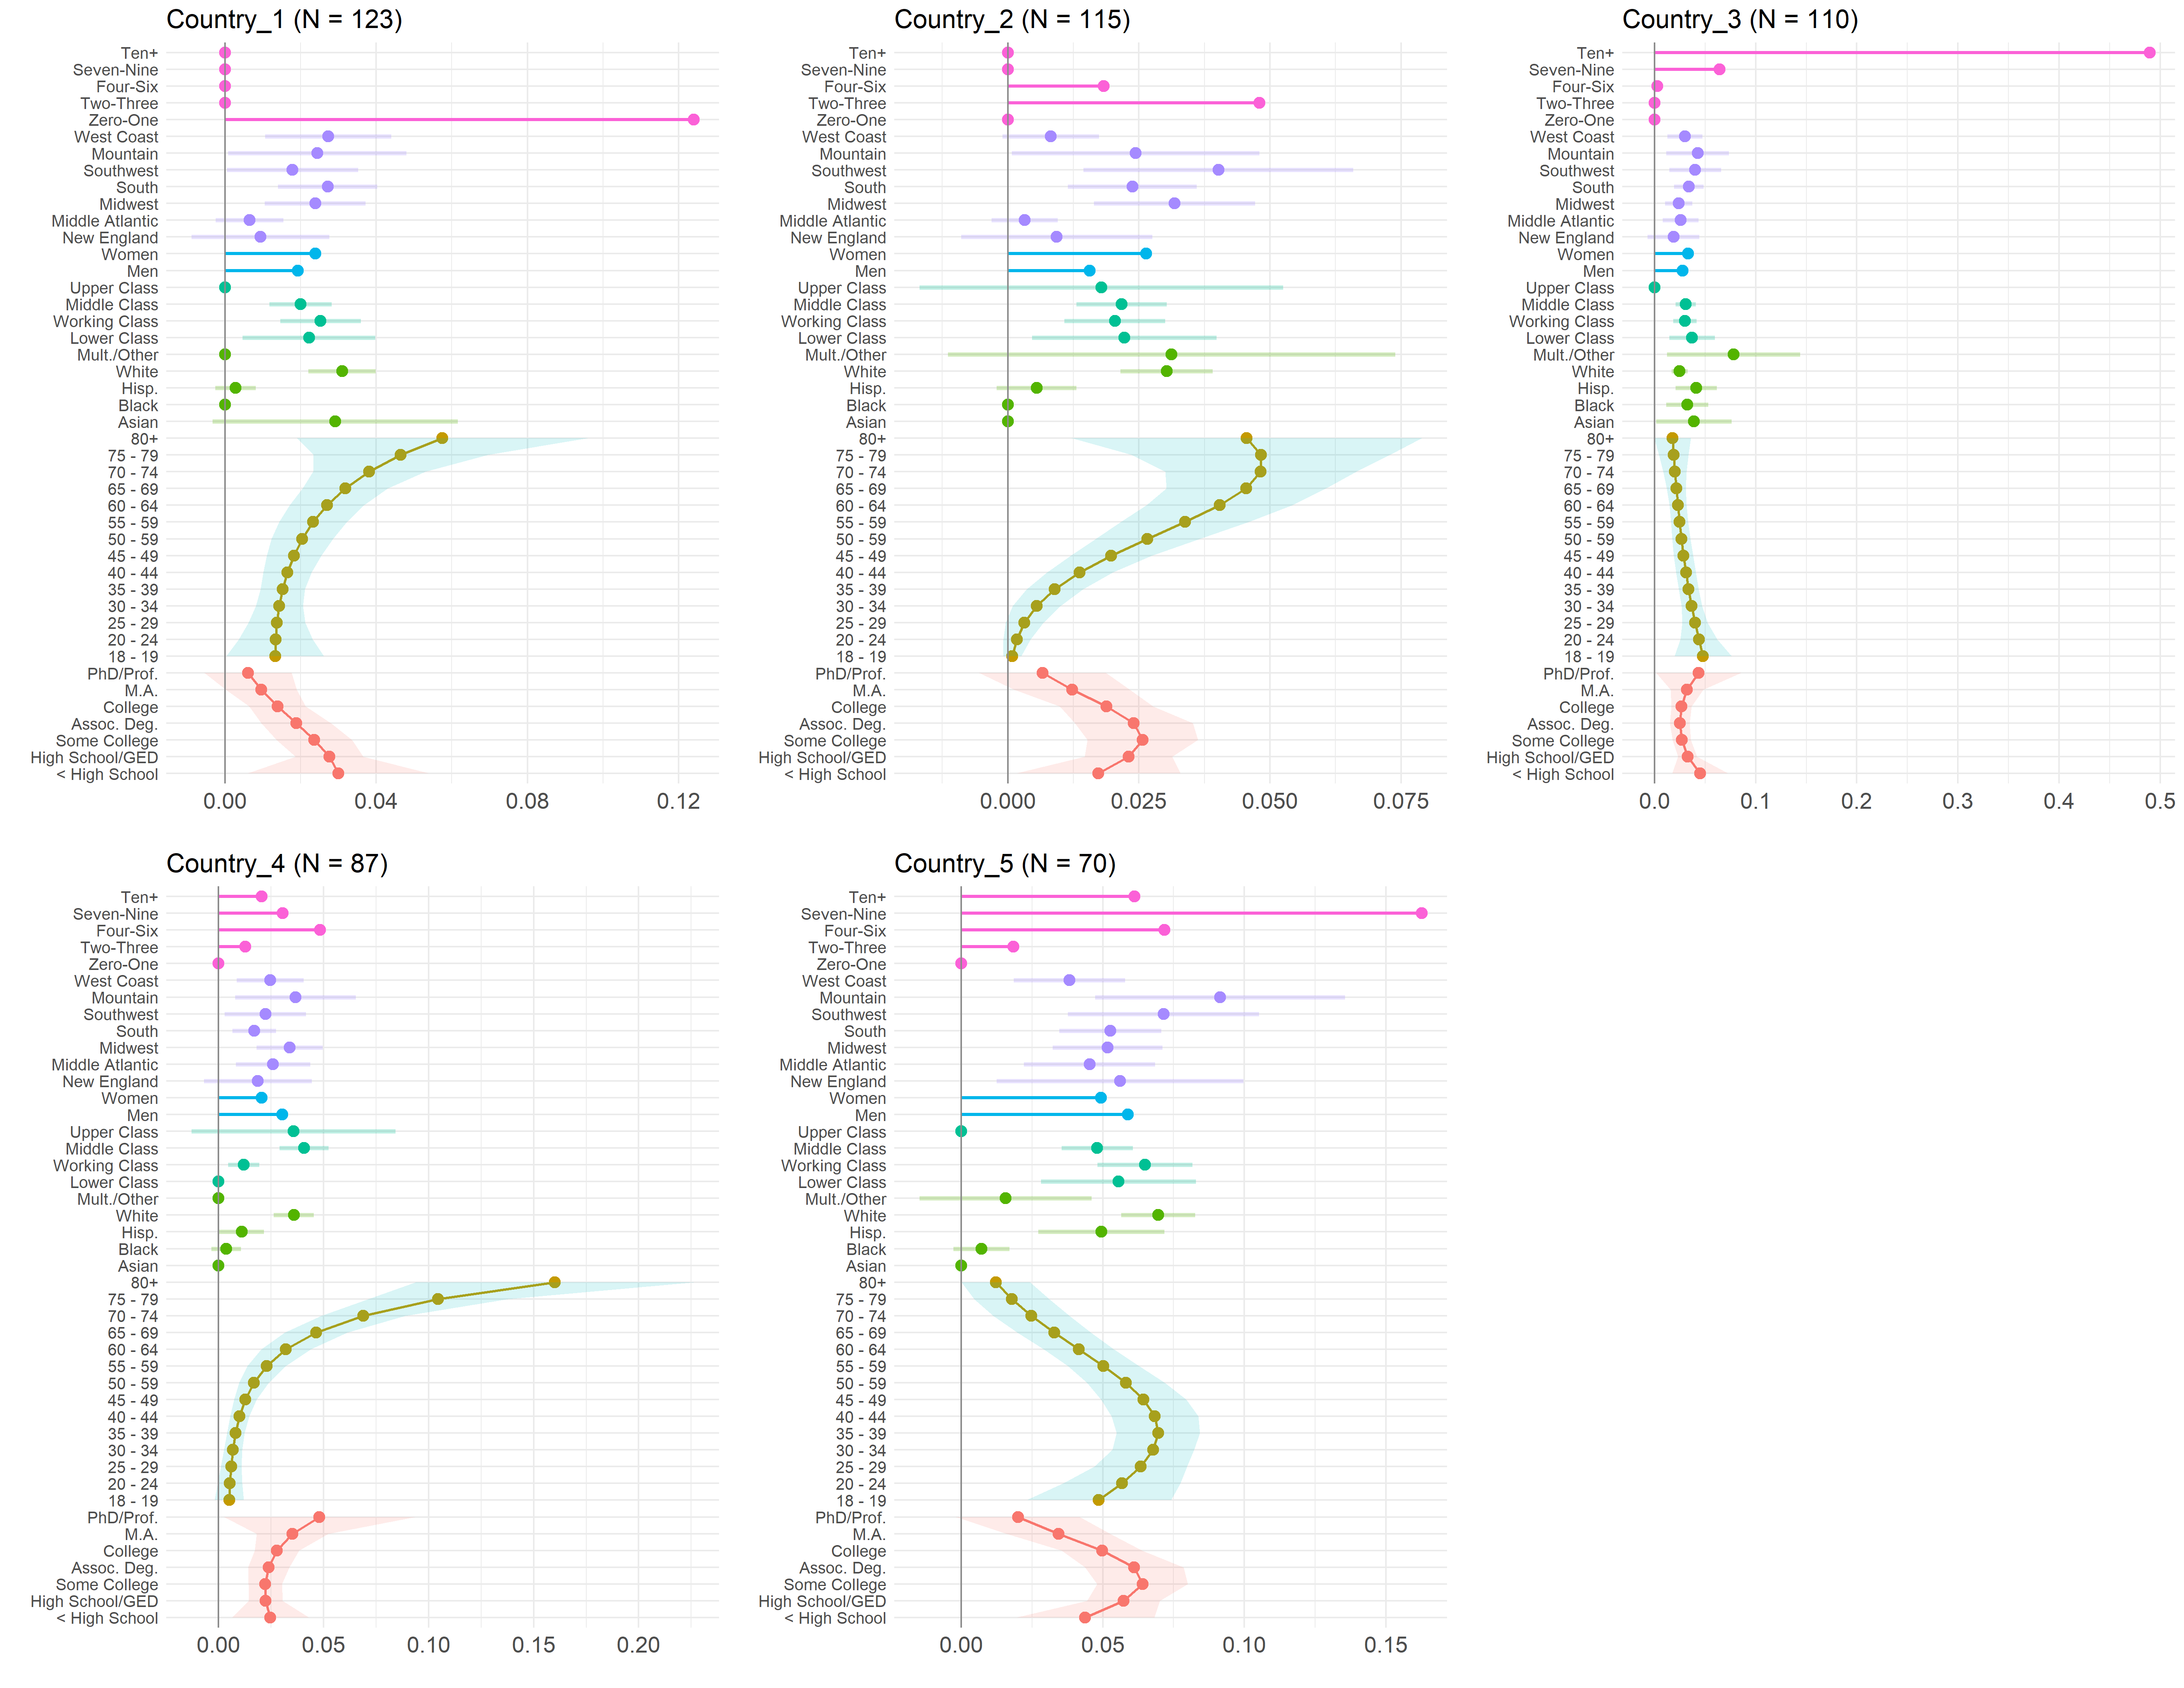
\includegraphics[width=1.0\textwidth]{figs/demog-plots/Country1.png}
        \caption{}
        \label{fig:Country1}
    \end{subfigure} 
     \begin{subfigure}[b]{0.8\textwidth}
        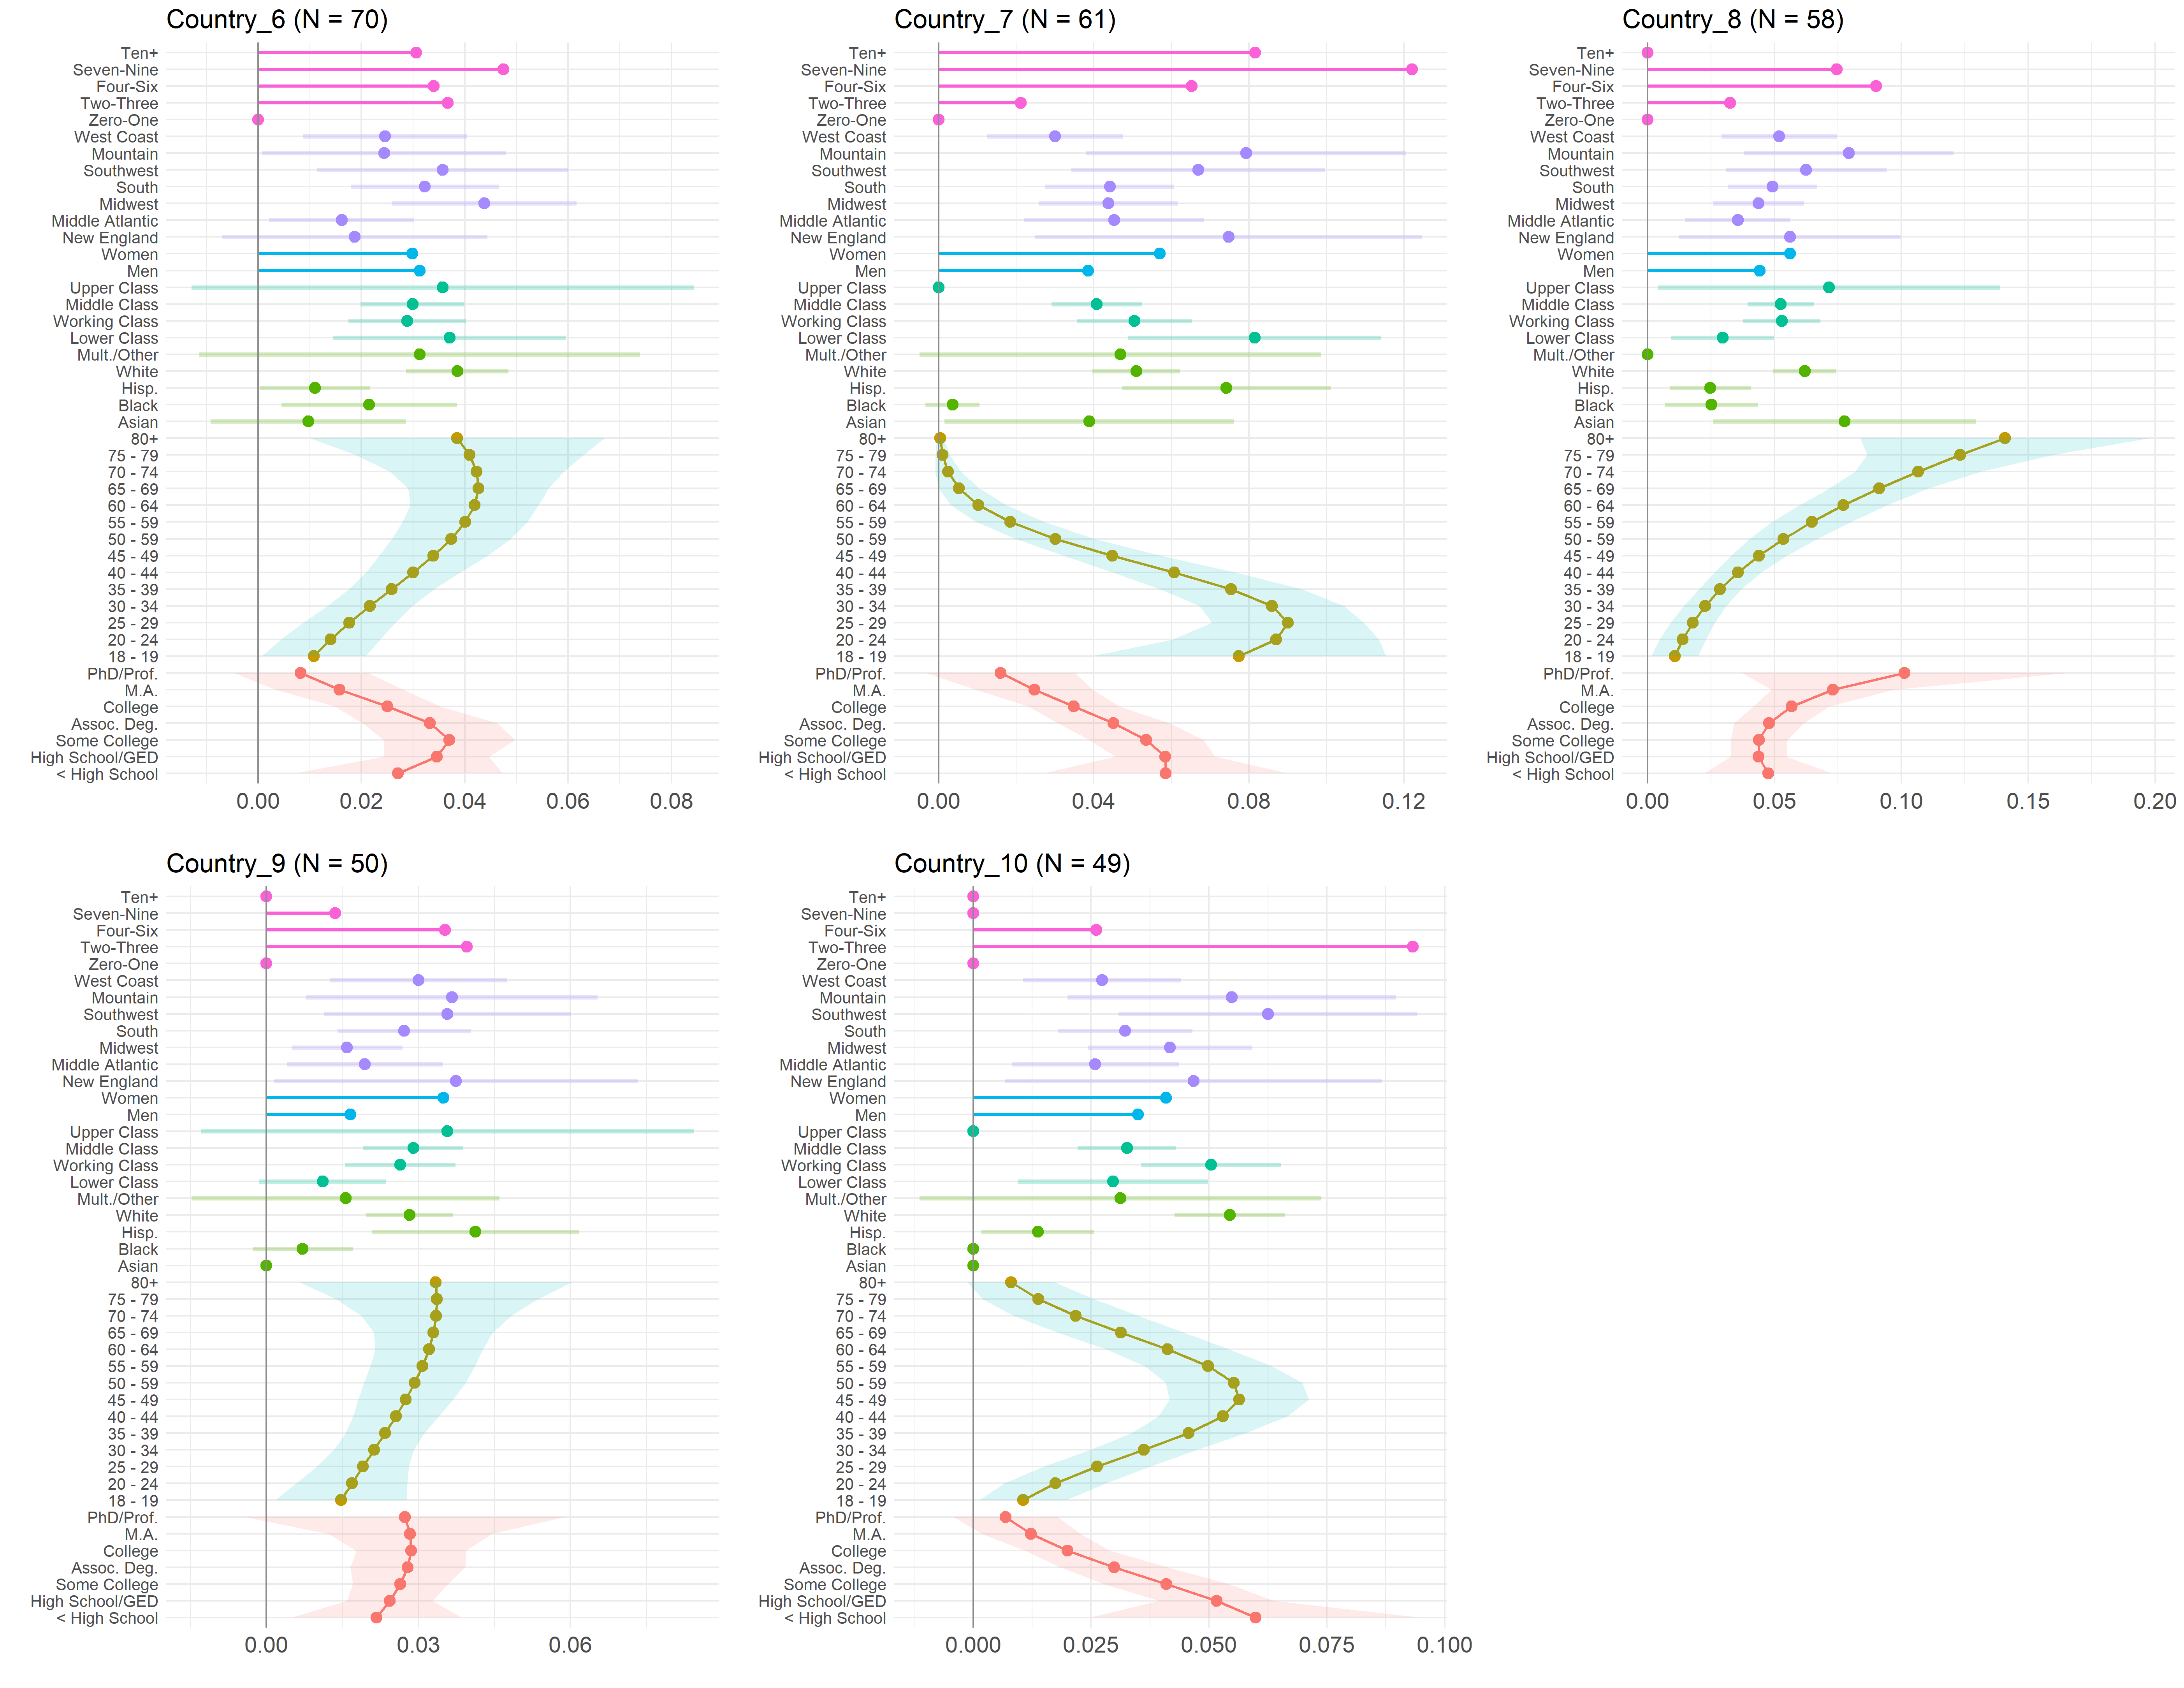
\includegraphics[width=1.0\textwidth]{figs/demog-plots/Country2.png}
        \caption{}
        \label{fig:Country2}
    \end{subfigure}
     \caption{}
  \label{fig:Country}
 \end{figure}